%%%%%%%%%%%%%%%%%%%%%%%%%%%%%%%%%%%%%%%%%%%%%%%%%%%%%%%%%%%%%%%%%%%%%%%%%%%%%%%%
%2345678901234567890123456789012345678901234567890123456789012345678901234567890
%        1         2         3         4         5         6         7         8

\pdfoutput=1
\pdfobjcompresslevel=0
\documentclass[letterpaper, 10 pt, conference]{ieeeconf}  % Comment this line out
                                                          % if you need a4paper
%\documentclass[a4paper, 10pt, conference]{ieeeconf}      % Use this line for a4
                                                          % paper

\IEEEoverridecommandlockouts                              % This command is only
                                                          % needed if you want to
                                                          % use the \thanks command
\overrideIEEEmargins
% See the \addtolength command later in the file to balance the column lengths
% on the last page of the document

%\usepackage[letterpaper, margin=0.75in]{geometry}
\usepackage{times}
\usepackage[utf8]{inputenc}
\usepackage{xcolor}
\usepackage{amsmath}

% Changed proof and theorem style to something I like better
% editor can change later if desired
\let\proof\relax
\let\endproof\relax

\usepackage{amsthm}
\usepackage{amsfonts}
\usepackage{amssymb}
%\usepackage{enumitem}
\usepackage{graphicx}
\usepackage{float}
\usepackage[justification=centering]{caption}
%\usepackage{subcaption}
%\allowdisplaybreaks
%\usepackage{longtable}
\usepackage{tikz}
%\usetikzlibrary{shapes,arrows,positioning,calc}
%\usetikzlibrary{cd}
%\usepackage{algorithmic}
%\usepackage{cite}
\usepackage[noadjust]{cite}
%\usepackage{verbatim}
%\usepackage[lofdepth,lotdepth,caption=false]{subfig}
%\usepackage{fancyhdr}
\usepackage{hyperref}
%\usepackage{xspace}
%\usepackage{braket}
%\usepackage{setspace}
\usepackage{comment}
\usepackage{tabularx}



%---Max's Definitions and Commands------------------------------------------------------
\newcommand{\R}{\mathbb{R}}
\newcommand{\Rnneg}{\R_{\geq 0}}
\newcommand{\Rpos}{\R_{>0}}
\newcommand{\C}{\mathbb{C}}
\newcommand{\Z}{\mathbb{Z}}
\newcommand{\N}{\mathbb{N}}
\DeclareMathAlphabet{\mymathbb}{U}{BOONDOX-ds}{m}{n}
\newcommand{\1}{\mymathbb{1}}
\newcommand{\0}{\mymathbb{0}}
\DeclareMathOperator*{\argmax}{argmax}
\DeclareMathOperator*{\argmin}{argmin}
\DeclareMathOperator{\var}{var}
\DeclareMathOperator{\cov}{cov}
\DeclareMathOperator{\diag}{diag}
\DeclareMathOperator{\spec}{spec}
\DeclareMathOperator{\tr}{tr}
\DeclareMathOperator{\avg}{avg}
\DeclareMathOperator{\supp}{supp}
\DeclareMathOperator{\sech}{sech}
\newcommand{\W}{\mathcal{W}}
\newcommand{\K}{\mathcal{K}}
\newcommand{\M}{\mathcal{M}}
\newcommand{\bbW}{\mathbb{W}}
\newcommand{\cJ}{\mathcal{J}}
\newcommand{\D}{\mathfrak{D}}

% Note conflict with Bassam's parentheses
%\newcommand{\lb}{\langle}
%\newcommand{\rb}{\rangle}
\newcommand{\lp}{\left(}
\newcommand{\rp}{\right)}
\newcommand{\of}{\circ}
\newcommand{\red}{\color{red}}
\newcommand{\half}{\frac{1}{2}}

\newcommand{\tcr}[1]{{\color{red} #1}}

\theoremstyle{plain}
\newtheorem{thm}{Theorem}%[chapter]
\newtheorem{lem}[thm]{Lemma}%[chapter]
\newtheorem{cor}[thm]{Corollary}%[chapter]
\newtheorem{prop}[thm]{Proposition}
\theoremstyle{definition}
\newtheorem{defn}[thm]{Definition}%[chapter]
\newtheorem{exmp}{Example}
\theoremstyle{remark}
\newtheorem*{rmk}{Remark}
\newtheorem*{sktch}{Sketch of Proof}
\newenvironment{sketch}{\begin{sktch}}{\hfill $\qed$ \end{sktch}}

\newtheorem{problem}[thm]{\bf Problem}


% The following packages can be found on http:\\www.ctan.org
%\usepackage{graphics} % for pdf, bitmapped graphics files
%\usepackage{epsfig} % for postscript graphics files
%\usepackage{mathptmx} % assumes new font selection scheme installed
%\usepackage{times} % assumes new font selection scheme installed
%\usepackage{amsmath} % assumes amsmath package installed
%\usepackage{amssymb}  % assumes amsmath package installed

\title{\LARGE \bf
Continuum Swarm Tracking Control: A Geometric Perspective in Wasserstein Space
}

%\author{ \parbox{3 in}{\centering Huibert Kwakernaak*
%         \thanks{*Use the $\backslash$thanks command to put information here}\\
%         Faculty of Electrical Engineering, Mathematics and Computer Science\\
%         University of Twente\\
%         7500 AE Enschede, The Netherlands\\
%         {\tt\small h.kwakernaak@autsubmit.com}}
%         \hspace*{ 0.5 in}
%         \parbox{3 in}{ \centering Pradeep Misra**
%         \thanks{**The footnote marks may be inserted manually}\\
%        Department of Electrical Engineering \\
%         Wright State University\\
%         Dayton, OH 45435, USA\\
%         {\tt\small pmisra@cs.wright.edu}}
%}

\author{Max Emerick and Bassam Bamieh% <-this % stops a space
%\thanks{This work was not supported by any organization}% <-this % stops a space
\thanks{M. Emerick and B. Bamieh are with the Department of Mechanical Engineering,
		University of California, Santa Barbara, USA
        {\tt\small memerick@ucsb.edu, bamieh@ucsb.edu}}%
}


\begin{document}



\maketitle
\thispagestyle{empty}
\pagestyle{empty}


%%%%%%%%%%%%%%%%%%%%%%%%%%%%%%%%%%%%%%%%%%%%%%%%%%%%%%%%%%%%%%%%%%%%%%%%%%%%%%%%
\begin{abstract}
We consider a setting in which one swarm of agents is to service or track a second swarm, and formulate an optimal control problem which trades off between the competing objectives of servicing and motion costs. We consider the continuum limit where large-scale swarms are modeled in terms of their time-varying densities, and where the Wasserstein distance between two densities captures the servicing cost. We show how this non-linear infinite-dimensional optimal control problem is intimately related to the geometry of Wasserstein space, and provide new results in the case of absolutely continuous densities and constant-in-time references. Specifically, we show that optimal swarm trajectories follow Wasserstein geodesics, while the optimal control tradeoff determines the time-schedule of travel along these geodesics. We briefly describe how this solution provides a basis for a model-predictive control scheme for tracking time-varying and real-time reference trajectories as well.
\end{abstract}


%%%%%%%%%%%%%%%%%%%%%%%%%%%%%%%%%%%%%%%%%%%%%%%%%%%%%%%%%%%%%%%%%%%%%%%%%%%%%%%%
\section{Introduction}

%1. Motivate problem in general
Low-cost sensing, processing, and communication hardware is driving the use of autonomous robotic swarms in diverse settings, including emergency response, transportation, logistics, data collection, and defense.
%\cite{Gautam2012,Cortes2017}.
%(\cite{Arai2002,Gautam2012,Demetriou2009})
Large swarms in particular can have significant advantages in efficiency and robustness. 
%However, as swarms scale in size it becomes increasingly difficult to plan and coordinate motion between agents. 
For sufficiently large swarms, modeling the swarm as a density distribution over the domain (i.e. as a continuum) provides a significant model reduction as well as improved insight into the global behavior of the swarm. Thus, the development of effective motion planning and control strategies for systems of distributions is a problem of interest.
%This effectively discards ``microscopic'' information pertaining to individual agents' states and identities while retaining ``macroscopic'' about how the swarm is distributed overall. This provides a significant model simplification and in many situations where we would apply large-scale swarms, this is all we really care about anyway.


%2. Talk about other approaches, cite literature
%{\red Must cite all the most relevant work}
%It has become apparent that the 
One natural mathematical setting in which to study these continuum swarm problems is the {\em Wasserstein space} of optimal transport theory. This space equips the set of normalized distributions over a domain with the {\em Wasserstein distance} -- a metric based on the cost of transport whose utility lies largely in the fact that it respects the topology of the underlying physical space\footnote{Compare, for example, the $L^p$ distance, which can be arbitrarily sensitive to spatial perturbations.}. In recent years, numerous approaches have been taken to swarm control using the Wasserstein distance and other tools from optimal transport theory. These works fall into two main approaches: one based on distributed optimization, and one based on optimal control. This work falls into the latter category.

In the distributed optimization approach, each agent communicates and acts locally to steer the entire swarm towards a given target distribution. The most relevant works here include \cite{Bandyopadhyay2014,Krishnan2018a,Inoue2021}. This approach has the advantage of being decentralized, and thus balancing the computation and communication loads in a way that is desirable in a practical implementation. However, these approaches have also been limited in their treatment of the objective and constraints: they seek to converge to the target distribution while minimizing the transport distance. In a real-world setting, it is desirable to have a model that can accommodate more general behaviors, especially since convergence to a target distribution is not always possible.
%Krishnan and Mart{\'i}nez - Optimal transport for distributed control. Steer toward desired formation. No optimal control. Cite other works?
%Banyopadhyay - Swarm guidance with optimal transport. Distributed. Steer toward desired formation. No optimal control. Cite other works?
%Inoue - Optimal transport-based coverage control. Believe distributed. No optimal control. Show solution generalizes and improved upon voronoi-based methods.
%Ferrari - Distributed optimal control. Nothing about Wasserstein or optimal transport. Don't cite.
%Elamvazhuthi - Optimal control of swarm distributions. Modeling via advection-reaction-diffusion PDE. No wasserstein/optimal transport. Don't cite.

On the other hand, in the optimal control approach, a central planner controls the entire swarm to minimize a given cost function. This approach has the advantages of being able to accommodate more general objectives and constraints and yielding greater insight into the nature of optimal swarm behavior generally. While the solutions here are centralized and thus impractical for a large-scale implementation, one expects that the insight gained from this approach will ultimately lend tools to design better distributed swarm control algorithms.

There is a large recent literature on optimal control in Wasserstein spaces, with the most relevant works in the area of multi-agent systems including \cite{Fornasier2014,Carrillo2014,Bonnet2019,Bonnet2019a, Bonnet2021,Bongini2017,Gangbo2008,Jimenez2020,Burger2021}. These works focus primarily on the analytic aspects of the problem such as existence and uniqueness of solutions and necessary conditions for optimality. They also focus on systems governed by various types of nonlocal PDEs which arise in connection with mean-field models for self-organizing swarms.

\begin{comment}
	In \cite{Fornasier2014} and \cite{Carrillo2014}, optimal control problems based on continuum models are derived for multi-agent systems.
	%While these works use the Wasserstein distance to prove convergence of discrete models to their continuum counterparts, the optimal control problems are not posed explicitly in the Wasserstein space.
	In \cite{Bonnet2019}, a maximum principle is proven for optimal control problems in Wasserstein space.
	In \cite{Bonnet2019a} and \cite{Bonnet2021}, this maximum principle is extended to optimal control problems with additional constraints.
	In \cite{Bongini2017}, a different maximum principle is proven for systems with coupled ODE/PDE dynamics.
	In \cite{Gangbo2008} and \cite{Jimenez2020}, the value functions of certain optimal control problems are characterized as viscosity solutions to respective Hamilton-Jacobi-Bellman equations.
	In \cite{Burger2021}, first-order optimality conditions (in the KKT-sense) are investigated in the Wasserstein space.
	%Fornasier and Solombrino - Mean-field optimal control. Derive continuum model for multi-agent systems. Nonlocal PDE. I beleive they use optimal transport for convergence and don't pose the problem explicitly in the wasserstein space. (Carrillo et. al. I think similar in scope).
	%Bonnet - Extends Bonnet and Rossi paper to systems with additional constraints
	%Bonnet and Rossi - Proves a Pontryagin maximum principle for optimal control problems in wasserstein space. Generalizes our problem with a more general cost function and a nonlocal transport PDE. Could potentially be used to prove existence/uniqueness for our problem.
	%Bonnet and Frankowska - another extension of Bonnet and Rossi for further constrained problems.
	%Jimenez et. al. - Similar but distinct problem. Different cost function, not for tracking. Characterize the value function as a viscosity solution of the Hamilton-Jacobi-Bellman equation.
	%Gangbo Nguyen Tudorascu - Existence of viscosity solutions to HJB equation in Wasserstein space.
	%Burger - Mean-field optimal control and optimality conditions in Wasserstein space. Derive PDE-based optimal control problem. Nonlocal PDE with Bolza-type cost. Possibly generalizes our work.
	%Bongini et al - Mean-field pontryagin maximum principle for Wasserstein space. Nonlocal coupled ODE/PDE constraints.
	These works are all fairly technical and abstract. They focus primarily on the analytic aspects of the problem such as existence and uniqueness of solutions and necessary conditions for optimality. They also focus mainly on systems governed by various types of nonlocal PDEs which arise in connection with {\em mean-field} swarm models motivated by self-organizing behavior.
\end{comment}


%3. How does our work fit in? What are main contributions?
In this paper, we continue the investigation of a model for continuum swarm tracking control originally proposed in \cite{Emerick2022}. The approach we take is in line with the second group of approaches in that it is based on optimal control in Wasserstein space. However, it differs from these approaches in that it is primarily concerned with tracking as opposed to self-organization and that it uses more explicit models to obtain sharper results. In short, the focus of this work is to answer the question ``what principles underlie optimal motion planning and control in swarm-based tracking scenarios?'' In contrast to our previous work on this problem \cite{Emerick2022,Emerick2022a} which focused on the special case of swarms in one spatial dimension, this work is more general in that it treats swarms in $n$ dimensions (clearly $n$ = 1, 2, or 3 in a practical setting). In addition, this work takes a distinctively geometric approach, which not only provides more powerful tools for solving these problems but yields additional insight into the problem's underlying structure.
The main contributions of this paper are thus:
\begin{itemize}
	\item The introduction of several geometric tools for solving swarm tracking control problems,
	
	\item Analytic solutions to our model in the $n$-dimensional case where the swarm distribution is absolutely continuous and the reference distribution\footnote{In this paper we use the terms {\em density} and {\em distribution} synonymously.}  is static.
	%
	%\item Interpretations of these results and presentation of a case study that illustrates how optimal swarm behavior changes in more general scenarios.
\end{itemize}

We first introduce our problem formulation and present our main result. The rest of the paper is then devoted to developing the tools necessary to prove it.

%We first introduce some background, including the models this work is based on and the geometric tools that we will use to analyze these models. We then show how these models can be reformulated as geometric problems in Wasserstein space or in the space of transport maps. We use these reformulations to solve the problem in the case where the resource distribution is continuous and the demand distribution is static. We then provide some analysis of this solution and present a case study that demonstrates how behavior can change under more general assumptions.



%%%%%%%%%%%%%%%%%%%%%%%%%%%%%%%%%%%%%%%%%%%%%%%%%%%%%%%%%%%%%%%%%%%%%%%%%%%%%%%%
\section{Problem Formulation and Main Result}

In previous work \cite{Emerick2022} we proposed a model for swarm tracking control. Since this proposed model forms the basis of this work, we briefly review the problem formulation here. For a full development and motivation, see \cite{Emerick2022}.

The key feature of our proposed problem setting is that there are two distributions, which we refer to as {\em demand} and {\em resource} respectively. The demand can be mobile or stationary and represents either locations, facilities, or independently-controlled mobile robots that require supplies or services (e.g. data collection, communication). Resource agents are mobile and are able to service the needs of multiple demand components. Physical space is taken to be $\R^n$ where $n$ is a positive integer. Both the demand and resource distributions are modeled as time-varying density distributions
%\footnote{From a measure-theoretic point of view, these distributions are density functions of finite measures. However, in this model we use generalized functions to describe such densities instead, e.g., we speak of Dirac distributions rather than ``atomic measures''. For a formal treatment of generalized functions, see \cite{Gelfand1964}.}
over the domain, taking the form
\begin{equation}
	\mu(x,t) ~=~ c(x,t) ~+~ \sum_{i=1}^N m_i(t) \, \delta \big( x-p_i(t) \big) .
\end{equation}
Here, $x \in \R^n$ is the spatial location while $t \in [0,T]$ is the time. The function $c: \R^n \times [0,T] \to \Rnneg$ is the continuum portion of the density distribution while the summation is the discrete portion. The continuum portion describes a continuum approximation of a large swarm while the discrete portion describes $N$ discrete agents having mass $m_i$ at location $p_i$. In this work, we present results exclusively for continuum swarms, and so from here on we assume that $N = 0$. We also assume that both resource and demand distributions have been scaled to integrate to 1
\begin{equation}
	\int_{\R^n} R(x,t) \, dx ~=~ \int_{\R^n} D(x,t) \, dx ~=~ 1 .
\end{equation}
We then say that the resource and demand distributions are {\em normalized}, and denote the set of normalized distributions over $\R^n$ as $\D(\R^n)$. We also make the additional technical assumption that the resource and demand distributions are supported within a compact subset $\Omega \subset \R^n$ for all time.
%When we need to refer to it, $\Omega$ will denote a compact set containing the supports of $R$ and $D$ for all time.

The resource agents service the needs of the demand through an assignment process where each resource particle is assigned to a set of demand particles and vice versa. This coupling is called an {\em assignment kernel} and is one of the decision variables in our optimal control problem. The assignment kernel incurs an {\em assignment cost} which is related to the efficiency of the assignment. In our setting, the assignment cost is motivated by the cost of communication between resource and demand swarms, and we assume that the assignment is chosen to be optimal at each instant in time. This leads to an assignment cost of the form
\begin{equation}
	\begin{split}
		\W_2^2(R_t,D_t) ~=~ &\min_\K \, \int_{\R^n \times \R^n} \Vert x - y \Vert_2^2 ~ \K(x,y,t) \, dx \, dy \\
		& \quad \text{s.t.} \quad \textstyle{\int \K \, dy = R} \\
		& \quad \phantom{\text{s.t.}} \quad \textstyle{\int \K \, dx = D}
	\end{split}
\end{equation}
which is exactly the square of the 2-Wasserstein distance of optimal transport theory \cite{Santambrogio2015}.
Equipped with the 2-Wasserstein distance, the space of normalized distributions $\mathfrak{D}(\R^n)$ becomes a complete metric space, which we call {\em 2-Wasserstein space} and denote $\bbW_2(\R^n)$. An important fact is that the space $\bbW_2(\R^n)$ is a geodesic space, and we will denote a geodesic in this space by $\Gamma$.

It is important to note that while the Wasserstein distance is motivated in optimal transport theory as an actual {\em transport} (i.e. 
motion) cost, that is not the way it is used  here. In our setting, this distance reflects for example the cost of communication between 
two sets of agents which is proportional to some measure of distance between two agents assigned to each other. The actual physical 
motion cost of a swarm is quantified differently as we describe next. 

The equations of motion of the system are given by the {\em transport equation}
\begin{equation} \label{transport_eqn}
	\partial_t R(x,t) ~=~ - \nabla \cdot \big( V(x,t) \, R(x,t) \big)
\end{equation}
where $R(\cdot,t)$ is the state of the resource distribution\footnote{Since we deal with objects that are simultaneously curves in function space as well as spatiotemporal fields, we use notations like $R_t$ or $R(\cdot,t)$ interchangeably, depending on which viewpoint we wish to emphasize in a given context. Notations like $f$ or $f(\cdot)$ are also used interchangeably and refer to a whole function as an object, while the notation $f(t)$ refers to the evaluation of that function at the point $t$.} at time $t$ and $V$ is a time-varying vector field which is considered as the control input. We assume that $V$ is continuous $R_t$-almost everywhere to ensure existence and uniqueness of solutions on the support of $R_t$. The velocity field $V$ incurs a {\em motion cost} which is related to the total energy expended in the motion. In our setting, the motion cost is motivated by the aerodynamic drag on the swarm, which leads to a motion cost of the form
\begin{equation}
	\int_{\R^n} \left\| V_t(x) \right\|_2^2 R_t(x) \, dx .
\end{equation}
Notice that this is just the $R_t$-weighted $L^2$ norm of $V(\cdot,t)$. This will become important later on.

Lastly, we have an {\em objective function} which defines optimal behavior for the resource swarm. The objective function is given by the integral of the assignment cost plus the motion cost over the time horizon $[0,T]$. The assignment cost and the motion cost are competing objectives; If the assignment cost is large, then the two distributions are far apart in the 2-Wasserstein distance, but that cost can be made smaller at the expense of motion, and vice versa.  
To capture the tradeoff between assignment and motion costs, we use a weighting  parameter $\alpha$ to control the relative importance of the two costs. All in all, the proposed problem is to find the control which minimizes the total cost of a maneuver. The problem is stated formally as follows.

\begin{problem}[\em Original Formulation] 															\label{orig}
	%	The {\em original problem} is defined to be the following. 
	Given an initial resource distribution $R_0 \in \D(\R^n)$ and demand trajectory $D: [0,T] \to \D(\R^n)$, solve
	\begin{equation}
		\begin{aligned} 
			\min_{V} \int_0^T & \left[ \W_2^2 \big( R_t,D_t \big)  +\alpha \int_{\R^n} \left\| V_t(x) \right\|_2^2 R_t(x) \, dx \right] dt  \\
			\mbox{s.t.} \quad
			&\partial_t R(x,t) = -\nabla \cdot \big( R(x,t) \, V(x,t) \big) . \\
			%&R(\cdot,0) = R_0 \\
			%&\cG : (R_t,D,t) \mapsto V_t   .   
		\end{aligned}
		\label{orig_eq}
	\end{equation}
	where $\W_2$ is the 2-Wasserstein distance, $\alpha > 0$ is the trade-off parameter, and $T$ is the time horizon.
	%We call the variable $V$ the {\em control}, $R$ the {\em trajectory}, and $\cJ$ -- the value of the objective -- the {\em cost}. A {\em solution} is defined to be a minimizer $\bar{V}$, if one exists. We use the term ``optimal'' for those values of the variables associated with the solution (e.g. ``the optimal trajectory'' or ``the optimal cost'').
\end{problem}

As stated, this problem is a nonlinear, infinite-dimensional optimal tracking problem: $R$ plays the role of the state, $D$ the reference trajectory, and $V$ the control input. The assignment cost (given by $\W_2^2$) plays the role of the tracking error, while the motion cost (given by the integral over $\R^n$) the control energy. The transport equation is the dynamical constraint. 


%%%%%%%%%%%%%%%%%%%%%%%%%%%%%%%%%%%%%%%%%%%%%%%%%%%%%%%%%%%%%%%%%%%%%%%%%%%%%%%%
\subsection{Main Result}

The main result of this paper is the following.

\begin{thm} \label{main_thm}
	When $R_0$ is absolutely continuous and $D(\cdot,t) = D(\cdot)$ is constant in time, the solution to the original problem \eqref{orig_eq} is given implicitly by the feedback controller
	\begin{equation} \label{opt_controller}
		V(x,t) ~=~ -f(t) \, \big( x - \M_t(x) \big) / \alpha
	\end{equation}
	where
	\begin{equation}
		f(t) ~=~ \sqrt{\alpha} \tanh \left( (T-t) / \sqrt{\alpha} \right) ,
	\end{equation}
	and $\M_t$ is the optimal transport map taking $R_t$ to $D$. The trajectory generated by this control law is
	\begin{equation}
		R_t ~=~ \left[ (1-\sigma(t)) \, \mathcal{I} ~+~ \sigma(t) \, \M_0 \right]_\# R_0
	\end{equation}
	where $\mathcal{I}$ is the identity map on $\R^n$, $\#$ the pushforward\footnote{Note that this refers to the pushforward of a distribution in the measure-theoretic sense, not the pushforward of a tangent vector in the differential-geometric sense.}, and
	\begin{equation}
		\sigma(t) ~=~ 1 - \cosh \left( (T-t) / \sqrt{\alpha} \right) .
	\end{equation}
	In particular, the trajectory $R_t$ follows the Wasserstein geodesic $\Gamma(R_0,D)$ from $R_0$ to $D$.
	Furthermore, this solution attains the cost
	\begin{equation} \label{opt_cost}
		\cJ(R_0,T;\alpha;D) = \frac{1}{2} \W_2^2(R_0,D) \sqrt{\alpha} \tanh \lp T / \sqrt{\alpha} \rp ,
	\end{equation}
	where $\W_2$ is the 2-Wasserstein distance.
\end{thm}

This provides a complete characterization of optimal swarm behavior in the case where the resource distribution is absolutely continuous and the demand distribution is static. 

Even though the solution \eqref{opt_controller} is for the case of a static demand distribution, it can be used as the basis for a receding-horizon Model-Predictive Control (MPC) scheme for tracking time-varying and apriori unknown demand trajectories. In this control scheme, the optimal transport map to the current demand distribution is computed at each timestep, the optimal control is found, and this control is applied over a short period of time $\Delta t$ before the process is repeated. See \cite{Limon2008} for a reference on using this sort of control scheme to achieve tracking for time-varying trajectories.

%We also provide arguments for why this characterization fails when either of these assumptions fail.

The rest of this paper focuses on developing the tools necessary to demonstrate these results. However, note that this does {\em not} imply that our primary objective in developing these tools is solely to establish said results. From a theoretical standpoint, these tools are quite interesting and useful in their own right.


%%%%%%%%%%%%%%%%%%%%%%%%%%%%%%%%%%%%%%%%%%%%%%%%%%%%%%%%%%%%%%%%%%%%%%%%%%%%%%%%
\section{The Geometric Picture}

A central tool in this paper is a geometric reformulation of optimal transport theory which we apply to 
the original problem stated above. In this section, we present a brief outline of this geometric view following Otto~\cite{Otto2001}. 
An in-depth study of this geometry can also be found in~\cite{Ambrosio2005}.

Let $\bbW_2$ be the 2-Wasserstein space of compactly supported probability distributions  on $\R^n$. 
%The first space that we will be working in is the 2-Wasserstein space of distributions (compactly supported) on $\R^n$. We will denote this space $\bbW_2$ and refer to it simply as the {\em Wasserstein space}, taking the domain and assumptions as implied. The Wasserstein space is simply the space of normalized distributions $\mathfrak{D}(\cdot)$ equipped with the 2-Wasserstein distance $\W_2$. 
%Under our assumptions, 
$\bbW_2$ is a complete metric space, a geodesic space, and an infinite-dimensional Riemannian manifold (with boundary) \cite{Ambrosio2005}. We will use the notions of curves, continuity, tangent vectors, length, speed, and geodesics which are standard in these settings\footnote{Note that the speed of a curve in $\bbW_2$ often goes by the name ``metric derivative'' in the optimal transport literature.}. We will denote arbitrary objects in the space $\bbW_2$ by $\mu$, $\nu$, or $\gamma$. In our optimal control problem, the objects in this space will be $R_t$ and $D_t$.

Intrinsically, the tangent space $T_{\mu} \bbW_2$ is identified with the set of variations on the distribution $\mu$. Roughly, these variations take the form of signed distributions on $\R^n$ having zero total mass \cite{Otto2001}.
%These variations take the form of signed distributions on $\Omega$ having zero total mass. At the boundary (i.e. if $\mu$ is such that $\supp (\mu) \subsetneq \Omega$), there is the additional constraint that the variation be nonnegative on $\Omega \setminus \supp (\mu)$.
However, we also frequently generate curves in $\bbW_2$ via the transport equation
\begin{equation}
	\mu_t' ~=~ - \nabla \cdot (v_t \, \mu_t) ,
\end{equation}
and so it is natural to ask what the relation is between the intrinsic tangent vectors (i.e. the variations on $\mu_t$) and objects of the form $ - \nabla \cdot \big( v_t \, \mu_t \big)$. It turns out that every sufficiently regular curve can be generated via the transport equation, and thus we choose to identify the tangent space  $T_\mu \bbW_2$ with the set of objects $\{ - \nabla \cdot ( v \, \mu) \}$.

\begin{lem}[{\cite[Theorem~5.14]{Santambrogio2015}}] \label{tan_vel_lem}
	Let $\mu: [0,T] \to \bbW_2$ be an absolutely continuous curve. Then there exists a time-varying vector field $v: \R^n \times [0,T] \to \R^n$ such that the pair $(\mu,v)$ satisfies the transport equation \eqref{transport_eqn}. Furthermore, the speed of the curve $\mu$ is defined for almost all $t$ and satisfies
	\begin{equation} \label{tan_vel_lem_eq_eq}
		|\mu_t'|^2 ~=~ \Vert v(\cdot,t) \Vert_{L^2(\mu_t)}^2 ~:=~ \int_{\R^n} ||v(x,t)||_2^2 \, \mu(x,t) \, dx .
	\end{equation}
	Conversely, let $\mu: [0,T] \to \bbW_2$ be any curve. Then the existence of a velocity field $v$ with finite $L^2(\mu_t)$-norm which together with $\mu$ satisfies the transport equation \eqref{transport_eqn} implies that the curve $\mu$ is absolutely continuous and
	\begin{equation} \label{tan_vel_lem_ineq_eq}
		|\mu_t'|^2 ~\leq~ \int_{\R^n} ||v(x,t)||_2^2 \, \mu(x,t) \, dx .
	\end{equation}
	%{\red Small technicalities about $\mu_t$ and $v$ in the above result as well}
\end{lem}

In short, a curve $\mu$ is absolutely continuous\footnote{Note that in this paper we use two different notions of absolute continuity -- that for distributions and that for curves. We will try to be explicit about which we are using in a given context.} if and only if $|\mu_t'|$ is defined almost everywhere if and only if there exists a $v$ such that $(\mu,v)$ satisfy the transport equation.

%Observe that this lemma not only gives us a correspondence between continuous curves in $\bbW_2(\Omega)$ and solutions to the transport equation, but identifies the metric tensor in $\bbW_2(\Omega)$ for us as well
%\begin{equation}
%	\begin{split}
%		G &: T_\mu \bbW_2(\Omega) \times T_\mu \bbW_2(\Omega) \to \R \\
%		& : (\mu_1' , \mu_2') \mapsto \min_{\substack{\mu_1' = - \nabla \cdot ( \mu u) \\ \mu_2' = - \nabla \cdot ( \mu v)}} \big\langle u , v \big\rangle_{L^2(\mu)} .
%	\end{split}
%\end{equation}

In analogy with fluid mechanics, we call this setting -- where we study objects in $\bbW_2$ with dynamics given by the transport equation -- the {\em Eulerian} setting, because we study the evolution of the resource distribution as a spatiotemporal field. There is another setting -- the {\em Lagrangian} setting -- where we study the movements of individual particles as their position changes. In the Lagrangian setting, the central objects of study are the integral curves of the time-varying vector field $v$. Recall that the collection of all integral curves of $v$ gives us the so-called {\em flow map} $\phi$:
\begin{equation} \label{flow_eqn}
	\begin{split}
		\partial_t \phi(x,t) &= v(\phi(x,t),t) \\
		\phi(x_0,0) &= x_0 .
	\end{split}
\end{equation}
The two settings are related as follows.
\begin{lem}[{\cite[Theorem~4.4]{Santambrogio2015}}] \label{transport_pushforward_lem}
	Let $\mu_0 \in \bbW_2$ be an absolutely continuous initial distribution and $v: \R^n \times [0,T] \to \R^n$ be a sufficiently regular time-varying vector field.
	%Let $\mu:[0,T] \to \bbW_2$ be a absolutely continuous curve and $v: \R^n \times [0,T] \to \R^n$ be a time-varying vector field which is continuous $\mu_t$-almost everywhere.
	Then $(\mu, v)$ satisfy the transport equation \eqref{transport_eqn} if and only if
	\begin{equation} \label{transport_pushforward_eqn}
		\mu_t ~=~ \left[ \phi(\cdot,t) \right]_\# \mu_0 ,
	\end{equation}
	where $\phi$ is the flow map of $v$ and $\#$ is the pushforward.
	%{\red To get if and only if, we need $\mu_t$ to be continuous for every $t$. (See theorem 4.4 in Santambrogio).}
	%{\red Again, there are technicalities here in what sort of $\mu_t$ and $v$ are allowed.}
\end{lem}

Recall that at a fixed instant in time, $\phi(\cdot,t)$ defines a map from $\R^n$ to $\R^n$. Thus, we choose to formalize this second (Lagrangian) perspective around maps $\M: \R^n \to \R^n$. The only requirement that we put on these maps is that they be measurable, and we denote the set of measurable maps from $\R^n$ to $\R^n$ as $\text{Meas}(\R^n)$. We will typically denote an object in this set as $\M$ for ``measurable'' or ``map'', or $\phi$ if we are referring to the flow of a specific velocity field.

Clearly $\text{Meas}(\R^n)$ forms a vector space, and thus a manifold, with tangent space also equal to $\text{Meas}(\R^n)$. We denote an element in $T_\M \text{Meas}(\R^n)$ as $u$ and define $u := v \of \M$ in the spirit of the flow equation \eqref{flow_eqn}. We choose to endow this space with the weighted $L^2$ metric tensor
\begin{equation}
	\begin{split}
		g_\mu(u_1,u_2) &~:=~ \langle u_1,u_2 \rangle_{L^p(\bar{\mu})} \\
		&~:=~ \int_{\R^n} u_1^T(x) u_2(x) \, \bar{\mu}(x) \, dx
	\end{split}
\end{equation}
where $\bar{\mu}$ is a fixed reference distribution. In this case, $\text{Meas}(\R^n)$ also becomes an infinite-dimensional Riemannian manifold, which we denote $\mathbb{M}(\R^n , \bar{\mu})$. Note in particular that $\mathbb{M}(\R^n , \bar{\mu})$ is {\em flat}.

Now, Lemma \ref{transport_pushforward_lem} tell us that the pushforward operator $\#$ defines a map
\begin{equation}
	\begin{split}
		\# &: \text{Meas}(\R^n) \times \bbW_2 \to \bbW_2 \\
		&: (\M , \mu ) \mapsto \M_\# \mu .
	\end{split}	
\end{equation}
Observe that with our reference distribution $\bar{\mu}$ fixed, by identifying $\text{Meas}(\R^n) \times \{ \bar{\mu} \}$ with $\mathbb{M}(\R^n,\bar{\mu})$, the pushforward induces a map between manifolds
\begin{equation}
	\begin{split}
		\Pi_{\bar{\mu}} &: \text{Meas}(\R^n) \times \{ \bar{\mu} \} \to \bbW_2 \\
		&: \mathbb{M}(\R^n,\bar{\mu}) \to \bbW_2 \\
		&: \M \mapsto \M_\# \bar{\mu} .
	\end{split}
\end{equation}
The map $\Pi_{\bar{\mu}}$ is smooth and onto provided that the distribution $\bar{\mu}$ is absolutely continuous \cite{Otto2001}. It is in general, however, many-to-one. In the language of differential geometry, $\Pi_{\bar{\mu}}$ defines a {\em submersion} of $\mathbb{M}(\R^n,\bar{\mu})$ in $\bbW_2$. Restricted in the proper way, though, $\Pi_{\bar{\mu}}$ will actually define a {\em diffeomorphism}. We define a right inverse for $\Pi_{\bar{\mu}}$ as follows
\begin{equation}
	\begin{split} \label{right_inv_eqn}
		\Pi_{\bar{\mu}}^{-R} &: \bbW_2 \to \mathbb{M}(\R^n,\bar{\mu}) \\
		&: \nu \mapsto \argmin_{ \M ~:~ \nu = \M_\# \bar{\mu} \hspace{-4ex}} \Vert \M - \mathcal{I} \Vert_{L^2(\bar{\mu})} .
	\end{split}
\end{equation}
Observe that the image of $\nu$ under $\Pi_{\bar{\mu}}^{-R}$ is exactly the solution to the Monge problem of optimal transport theory, i.e. the optimal transport map from $\bar{\mu}$ to $\nu$. Recall that when $\bar{\mu}$ is absolutely continuous, a unique minimizer to the Monge problem is guaranteed to exist \cite[Theorem~1.22]{Santambrogio2015}. Thus the image of $\Pi_{\bar{\mu}}^{-R}$ is the set of optimal transport maps in $\mathbb{M}(\R^n,\bar{\mu})$. It is known that a transport map is optimal if and only if it is equal to the gradient of a convex function, and so, remarkably, the set of optimal transport maps is actually {\em independent of the distribution $\bar{\mu}$}. We denote this set -- the image of $\Pi_{\bar{\mu}}^{-R}$, the set of optimal transport maps -- as $\text{Opt}(\R^n)$. Since the set of convex functions forms a convex cone, this structure is preserved under the gradient operator (which is linear), and so $\text{Opt}(\R^n)$ also forms a convex cone. Thus $\text{Opt}(\R^n)$ also forms a manifold (with boundary). Since $\text{Opt}(\R^n)$ is convex, it inherits the geometry of the subspace that it resides in. Equipped with the same $L^2(\bar{\mu})$ metric tensor as $\text{Meas}(\R^n,\bar{\mu})$, we denote this manifold $\mathbb{O}(\R^n,\bar{\mu})$, and remark once again that it is flat. Thus $\Pi_{\bar{\mu}}$ and $\Pi_{\bar{\mu}}^{-R}$ define a diffeomorphism:
\begin{equation}
	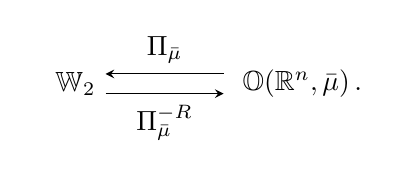
\begin{tikzpicture}[baseline={([yshift=-.5ex]current bounding box.center)}]
		\node at (-2,0) {$~~\mathbb{W}_2$};
		\node at (1,0) {$\mathbb{O}(\mathbb{R}^n,\bar{\mu}) \, .$};
		\draw [-stealth](-1.5,-0.125) -- (0,-0.125);
		\draw [-stealth](0,0.125) -- (-1.5,0.125);
		\node at (-0.75,0.425) {$\Pi_{\bar{\mu}}$};
		\node at (-0.75,-0.5) {$\Pi_{\bar{\mu}}^{-R}$};
	\end{tikzpicture}
\end{equation}
We now mention some properties of $\Pi_{\bar{\mu}}$ and its inverse. First, notice that since $\mathbb{O}(\R^n,\bar{\mu})$ is flat, $\Pi_{\bar{\mu}}^{-R}$ defines a coordinate chart (in fact, a global coordinate chart) on $\bbW_2$. Second, the differentials of $\Pi_{\bar{\mu}}$ and its inverse are given by
\begin{equation}
	\begin{split}
		d \Pi_{\bar{\mu}} &: T_\M \mathbb{O}(\R^n,\bar{\mu}) \to T_{\Pi_{\bar{\mu}}(\M)} \bbW_2 \\
		&: v \of \M \mapsto - \nabla \cdot \big( (\M_\# \bar{\mu}) \, v \big) ,
	\end{split}
\end{equation}
\begin{equation} \label{tangent_eqn}
	\begin{split}
		d \Pi_{\bar{\mu}}^{-R} &: T_{\nu} \bbW_2 \to T_{\Pi_{\bar{\mu}}^{-R}(\nu)} \mathbb{O}(\R^n,\bar{\mu}) \\
		&: \nu' \mapsto \argmin_{v ~:~ \nu' = - \nabla \cdot ( \nu v) \hspace{-5ex}} \Vert v \Vert_{L^2(\nu)} . \\
	\end{split}
\end{equation}
Note that in these expressions we have used the relations
\begin{multline}
	\langle u_1 , u_2 \rangle_{L^2(\bar{\mu})} ~=~ \langle v_1 \of \M , v_2 \of \M \rangle_{L^2(\bar{\mu})} \\
	~=~ \langle v_1 , v_2 \rangle_{L^2({\M}_\# \bar{\mu})} ~=~ \langle v_1 , v_2 \rangle_{L^2(\nu)} .
\end{multline}
There are three important facts here that we wish to point out. First, that the metric tensor in $\bbW_2$ is given by $g_\nu(s_1,s_2) = \langle v_1 , v_2 \rangle_{L^2(\nu)}$ where $s_1 = - \nabla \cdot ( \nu \, v_1 )$ and similarly for $s_2$. Second, that with this choice of metric tensor, $d \Pi_{\mu_0}$ defines an isometry between the tangent spaces of $\mathbb{O}(\R^n,\bar{\mu})$ and $\bbW_2$. Third, since we have $|\nu'| = \Vert v \Vert_{L^2(\nu)}$ from Lemma \ref{tan_vel_lem}, this choice of metric tensor does indeed generate the Wasserstein distance. Thus, to quote Otto \cite{Otto2001}, ``the best way to understand the geometry of $\bbW_2$ is that it is induced by a flat Riemannian space $\mathcal{O}(\R^n, \bar{\mu})$ via the Riemannian (i.e. metric tensor-preserving) submersion $\Pi_{\bar{\mu}}$.''

The last fact about $\Pi_{\bar{\mu}}$ that we wish to point out is that since vectors in the tangent space can be associated 1-1 with geodesics passing through the base point via the exponential map, $\Pi_{\bar{\mu}}$ and $\Pi_{\bar{\mu}}^{-R}$ take geodesics passing through $\M$ to geodesics passing through $\M_\# \bar{\mu}$ and vice versa. This can be used to recover the well-known formula for a geodesic in Wasserstein space from $\bar{\mu}$ to $\nu$
\begin{equation} \label{geodesic_eqn}
	\left[ (1-t) \, \mathcal{I} ~+~ t \, \Pi_{\bar{\mu}}^{-R}(\bar{\mu}) \right]_\# \bar{\mu} .
\end{equation}
This also means that $\Pi_{\bar{\mu}}^{-R}$ preserves the distance between $\bar{\mu}$ and any other distribution $\nu$:
\begin{multline}
	\W_2(\mu_0,\nu) ~=~ \Vert \M - \mathcal{I} \Vert_{L^2(\mu_0)} \\
	~=~ \big\Vert \Pi_{\mu_0}^{-R}(\nu) - \Pi_{\mu_0}^{-R}(\mu_0) \big\Vert_{L^2(\mu_0)} .
\end{multline}
Thus $\Pi_{\bar{\mu}}^{-R}$ can be intuitively conceptualized as a sort of ``flattening'' of $\bbW_2$ centered at $\bar{\mu}$.

%{\red This property of preserving geodesics means that this transformation has some strong structure to it. I'm thinking there must be a name for this sort of transformation in the literature. It's stronger than {\em conformal} but weaker than an {\em isometry}. The term {\em affine} is close, but is typically applied to a transformation from a manifold to itself. Ha, Riemannian submersion actually covers this, nevermind.}

%In the context of our optimal control problem, there are three obvious choices for $\bar{\mu}$. First, the initial distribution $R_0$. This gives the standard Lagrangian description of the system in terms of the flow $\phi$. Second, the current state of the system $R_t$. This gives a ``body coordinate frame'' for our system, but note that this is a time-varying transformation and so must be treated more carefully. Third, a ``standard distribution'', which is naturally chosen to be the uniform distribution over the unit volume $[0,1]^n$ and denoted $\mathcal{U}$. This last representation has the advantage of making our formulas work out nicely, and so we use it extensively in this work.

%When using transformations of this third type, we will use the notation $Q_\nu$ to denote the map such that $\nu = {Q_\nu}_\# \mathcal{U}$. This notation is in analogy with the {\em quantile function} of probability distributions in 1D. (The quantile function $Q_\nu$, while usually characterized as the inverse function of the cumulative distribution function, is also the unique monotone nondecreasing function with this property.) Representations of this form are very similar to those using $R_0$ (i.e. the standard Lagrangian description), but instead of labeling particles with their initial position $x_0$, this representation labels each particle with a unique index in $[0,1]^n$.

%Lastly, we note that when working in the Lagrangian setting, we will often find it convenient to work with an alternative representation of $\bbW_2(\Omega)$. Instead of representing a distribution $\mu$ as a density over $\Omega$, we will represent $\mu$ as a map $Q_\mu$ which pushes $\mathcal{U}$, the uniform distribution over the unit volume $[0,1]^n$, onto $\mu$, that is, $\mu = {Q_\mu}_\# \mathcal{U}$. Note that this is not a unique representation unless we enforce some  additional constraints on $Q_\mu$. These maps formally take values in the space of measurable isomorphisms from $[0,1]^n$ to $\Omega$, which we denote $\text{Meas} \big( [0,1]^n, \Omega \big)$. We will typically denote maps in this space with $Q$ in analogy with the quantile function of probability distributions in 1D\footnote{The quantile function, while usually characterized as the inverse function of the cumulative distribution function, is also the unique monotone nondecreasing function that pushes the uniform distribution over $[0,1]$ onto the probability distribution.}.
%Note that $\text{Meas}(\Omega)$ acts on $\text{Meas} \big( [0,1]^n, \Omega \big)$ in exactly the same way that it acts on $\bbW_2(\Omega)$. The transformations $\Pi$ and $\Pi^{-R}$ and their properties are the same, except that they are now centered at a map $Q_{\mu_0}$ instead of at a distribution $\mu_0$.
%Representing an object in $\bbW_2(\Omega)$ with an object in $\text{Meas} \big( [0,1]^n, \Omega \big)$ is akin to indexing each particle in the distribution with a value in $[0,1]^n$. When we use this parameterization in the Lagrangian setting we are essentially just taking particles that were originally labeled with their initial position $x_0$ and relabeling them with their index in $[0,1]^n$. The use of representations of this form is not because it is more powerful nor because is it mathematically more intuitive, but simply because it makes our formulas nice.



%\subsection{Continuum Models}

%The central concept that we work with is that of a {\em distribution}.

\begin{comment}
	\begin{defn}[Distributions]
		A {\em distribution} over $\Omega \subset \R^n$ is an object $\mu$ of the form%\footnote{From a measure theory point of view, these distributions are just density distributions of finite measures.}
		\begin{equation}
			\mu(x) ~=~ c(x) + \sum_{i=1}^N m_i \delta(x-p_i)
		\end{equation}
		where $x \in \Omega$, $c: \Omega \to \R$, $N \in \Z_{\geq 0}$, $m_i \in \Rpos$, $p_i \in \Omega$, and $\delta$ is the Dirac distribution. The first term is called the {\em continuous component}, and the second term is called the {\em discrete component}. A distribution is said to be {\em absolutely continuous} (hereafter, just {\em continuous}) if $N=0$, {\em discrete} if $c \equiv 0$, or {\em mixed} otherwise. A distribution $\mu$ is said to be {\em normalized} if
		\begin{equation}
			\int_\Omega \mu(x) \, dx ~=~ \int_\Omega c(x) \, dx ~+~ \sum_{i=1}^N m_i ~=~ 1 .
		\end{equation}
		We denote the {\em set of normalized distributions over $\Omega$} as $\D(\Omega)$.
	\end{defn}
\end{comment}

%A map can act on a distribution to give a new distribution called the {\em pushforward}.

\begin{comment}
\begin{defn}[Pushforward Distribution]
	Let $\mu$ be a distribution defined on some subset of $\R^n$ and let $\M: \R^n \to \R^m$ be a map. Then the {\em pushforward} of $\mu$ by $\M$, denoted $\M_\# \mu$, is a distribution on a subset of $\R^m$ such that
	\begin{equation}
		\int_A (\M_\# \mu)(y) \, dy = \int_{\M^{-1}(A)} \mu(x) \, dx
	\end{equation}
	for any set $A \subset \R^m$, where $\M^{-1}$ denotes the preimage.
\end{defn}
\end{comment}

%Intuitively, the pushforward can be thought of as a distribution formed by ``moving the mass in $\mu$ according to $\M$''. We will be interested in how distributions transform when acted on by time-varying vector fields. First, we define the {\em flow}.

\begin{comment}
	\begin{lem}
		Let $\mu$ be a distribution defined on $\Omega_1 \subset \R^n$ and let $\M: \Omega_1 \to \Omega_2 \subset \R^n$ be a smooth 1-1 mapping. Then the pushforward of $\mu$ by $M$ satisfies
		\begin{equation}
			(\M_\# \mu) \lp \M(x) \rp = \frac{\mu(x)}{|\det (\mathcal{D} \M(x))|}
		\end{equation}
		where $\mathcal{D}$ denotes the Jacobian.
	\end{lem}
	
	\begin{proof}
		The result is well-known. See e.g. the ``change of variables formula'' in Chapter 1 of \cite{Villani2009}.
	\end{proof}
\end{comment}

\begin{comment}
\begin{defn}[Flow of a Vector Field] \label{flow}
	Let $v: \R^n \times \R \to \R^n$ be a time-varying vector field. The {\em flow} of the vector field $v$ is a map $\phi : \R^n \times \R \to \R^n$ satisfying
	\begin{equation} \label{flow_eqn}
		\begin{split}
			\partial_t \phi(x,t) &= v(\phi(x,t),t) \\
			\phi(x_0,0) &= x_0 .
		\end{split}
	\end{equation}
	%{\red what assumptions do we make on $v$?}
\end{defn}
\end{comment}

%By defining the flow, we reserve $x$ as a coordinate by using $\phi$ for the position variable. The symbol $\phi(x_0,t)$ represents the position at time $t$ of the agent that started from $x_0$ at time $0$. Note that although we no longer keep track of the {\em identities} of individual agents, we can still {\em follow} individual agents over time via the flow. The flow gives us the swarm dynamics in the so-called {\em Lagrangian} perspective of fluid mechanics (that is, following individual agents as their position changes). There is also an expression for the swarm dynamics in the {\em Eulerian} viewpoint, describing the time-evolution of the entire density field. The ``Eulerian'' dynamics are given by the so-called {\em transport equation} (sometimes also referred to as the {\em advection equation} or {\em continuity equation}).

%If particles of mass at location $x$ move according to $\dot{x} = v(x)$, then $\phi(x,t)$ tells us the location at time $t$ of the particle that started from location $x$ at time $t=0$. The flow expresses the swarm dynamics in the {\em Lagrangian} perspective of fluid mechanics -- that is, following individual particles of mass as their position changes. There is also an expression for the swarm dynamics in the {\em Eulerian} viewpoint -- describing the time-evolution of the overall mass distribution -- given by the {\em transport equation}.

\begin{comment}
\begin{defn}[Transport Equation] \label{transport}
	Let $\mu_0 \in \mathfrak{D}(\Omega)$, $\Omega \subset \R^n$ be an initial distribution and $v: \Omega \times [0,T] \to \R^n$ be a time-varying velocity field. The {\em transport equation} is the following partial differential equation
	\begin{equation} \label{transport_eqn}
		\partial_t \mu(x,t) ~=~ - \nabla \cdot \big( v(x,t) \,\mu(x,t) \big) .
	\end{equation}
	A {\em solution} to the transport equation is a map $\mu_t : [0,T] \mapsto \mathfrak{D}(\Omega)$ that satisfies \eqref{transport_eqn} in some suitable weak sense
	%(specifically, in the distributional sense, $\mu_t$-almost everywhere for almost all time)
	with boundary conditions given by $\mu(x,0) = \mu_0(x)$ and $V = 0$ on $\partial \Omega$.
	%{\red perhaps $v$ needs to be continuous on sets where $\mu_t$ has nonvanishing mass?}
	{\red There are some technicalities in here regarding what sort of restrictions we put on $\mu_t$ and $v$. Saving these issues for later.}
\end{defn}
\end{comment}



%The interpretation here is that if the particles of mass in a distribution are advected according to the dynamics $\dot{x} = v(x)$ then the overall distribution evolves according to the transport equation.

%\begin{proof}
%	This is a foundational result in continuum mechanics -- see e.g. Section 5.3 in Mase \cite{Mase2009}.
%\end{proof}

%Equations \eqref{flow_eqn} and \eqref{transport_eqn} are the foundation of the model that we will use throughout this work.


%\subsection{Optimal Transport}

%Optimal transport theory has provided many useful tools for modeling and analyzing the motions of distributions in a physical space. This section reviews many of the key results from this field that we will use throughout this work. We proceed rather informally and without proof, attempting to build a little intuition rather than give a rigorous development. Indeed, optimal transport theory can be a technical discipline and a rigorous development is well-outside the scope of this work. For references on the material in this section, one can consult any of the classic texts on the subject by Santambrogio \cite{Santambrogio2015}, Ambrosio \cite{Ambrosio2005}, or Villani \cite{Villani2021,Villani2009}.

\begin{comment}
In short, the optimal transport problem seeks to find the most efficient way to transform one distribution of mass into another. The situation is formalized as follows. Suppose that we have an initial distribution of mass $\mu$, where $\mu(x)$ specifies the density of mass at location $x$, and we wish to transform it into a target distribution $\nu$, with a density $\nu(y)$ (we assume that the two distributions have the same total mass). One way to do this is by specifying a map $\M:x \mapsto y$ which takes the distribution $\mu$ and creates a new distribution by taking the mass from location $x$ and moving it to location $y$. 

Perhaps the most straightforward way to formalize the optimal transport problem is to define a function $c(x,y)$ representing the cost of moving mass from location $x$ to location $y$, and then minimize the total cost over all maps $\M$ that transport $\mu$ to $\nu$. This formulation is often referred to as the {\em Monge problem}.

\begin{defn}[Monge Problem] \label{mp}
	Let $\mu,~\nu \in \mathfrak{D}(\Omega)$, $\Omega \subset \R^n$ be two distributions and $c(x,y): \R^n \times \R^n \to \Rnneg$ be a cost function. The {\em Monge Problem} is to find the map of minimum cost transporting $\mu$ to $\nu$.
	\begin{equation} \label{mp_eqn}
		\begin{split}
			&\min_\M \, \int_{\Omega} c \lp x,\M(x) \rp \mu(x) \, dx \\
			& \quad \text{s.t.} \quad \M_\# \mu = \nu
		\end{split}
	\end{equation}
	The minimizer $\bar{\M}$ is termed the {\em optimal transport map} and the value of the objective is termed the {\em transport cost} and is written $\cJ$.
\end{defn}

%While the Monge problem plays an important role in optimal transport theory, it is difficult to solve. It is nonconvex, and solutions are not even guaranteed to exist\footnote{For example, consider $\mu$ to be a Dirac distribution. Since the mass in $\mu$ can only be sent to one location, it is obvious that there is no solution unless $\nu$ is also a Dirac distribution.}. These issues are remedied by another formulation, the so-called {\em Kantorovich Problem}. Instead of seeking a map between the distributions, the Kantorovich problem seeks a more general coupling called a {\em plan}.

The optimal transport map will play a central role in this work. However, while we won't go into details here, the Monge problem is badly behaved for certain classes of distributions, and this motivates another formulation of the optimal transport problem called the {\em Kantorovich problem} that the reader should be made aware of.

\begin{defn}[Kantorovich Problem] \label{kp}
	Let $\mu,~\nu \in \mathfrak{D}(\Omega)$, $\Omega \subset \R^n$ be two distributions and $c(x,y): \R^n \times \R^n \to \Rnneg$ be a cost function. The {\em Kantorovich Problem} is to find the plan of minimum cost transporting $\mu$ to $\nu$.
	\begin{equation} \label{kp_eqn}
		\begin{split}
			& \min_\K \, \int_{\Omega \times \Omega} c(x,y) \, \K(x,y) \, dx \, dy \\ %= \argmin_\K \langle C , \K \rangle \\
			& \quad \text{s.t.} \quad {\Pi_x}_\# \K = \mu \\
			& \quad \phantom{\text{s.t.}} \quad {\Pi_y}_\# \K = \nu
		\end{split}
	\end{equation}
	where $\Pi_x : (x,y) \to x$ and $\Pi_y : (x,y) \to y$ are the projections onto $x$ and $y$, respectively. The minimizer $\bar{\K}$ is termed the {\em optimal transport plan} and the value of the objective is again termed the {\em transport cost} and written $\cJ$. %{\red Give the inner product form here?}
\end{defn}

Whereas the Monge problem specifies {\em where} the mass at each point $x$ is transported, the Kantorovich problem specifies {\em how much} mass is transported from each point $x$ to each point $y$. In this way, the Kantorovich problem is more general, because one is allowed to ``split mass'' by sending it to multiple locations.
%A transport plan $\K$ can be interpreted as a joint distribution having the source and target distributions as marginals.
\end{comment}

\begin{comment}
	%This formulation yields a number of advantages over the Monge problem. First, the Kantorovich problem consists of a linear objective function under linear constraints and is thus an infinite-dimensional linear program, which can be solved by established methods. Second, solutions are always guaranteed to exist. Third, if the Monge problem is solvable, its solutions can be recovered from the solution to the Kantorovich problem as follows.
	
	Solution to the Kantorovich problem are always guaranteed to exist. If the Monge problem has a solution, its solutions can be recovered from the solution to the Kantorovich problem as follows.
	
	\begin{lem} \label{map_recovery}
		When $\mu$ is absolutely continuous, the optimal transport plan $\bar{\K}$ solving \eqref{kp_eqn} takes the form
		$(\mathcal{I}, \bar{\M})_\# \mu$, where $\mathcal{I}$ is the identity map on $x$ and
		%\begin{equation}
		%	\bar{\K}(x,y) = \delta \big(y - \bar{\M}(x)\big) \frac{\mu(x)}{\sqrt{1 + \big(M'(x)\big)^2}} % only works for 1D
		%\end{equation}
		$\bar{\M}$ is the optimal transport map solving \eqref{mp_eqn}.
		%{\red Bassam asks for more explicit formula... I haven't seen one in the literature but I think it would be something like
			%\begin{equation}
			%	\bar{\K}(x,y) ~=~ \delta(y - \bar{\M}(x)) \frac{\mu(x)}{\sqrt{1 + \det^2 \big( \mathcal{D} \bar{\M}(x) \big)}}
			%\end{equation}
			%}
	\end{lem}
	
	\begin{proof}
		See Theorem 1.17 in Santambrogio \cite{Santambrogio2015}.
	\end{proof}
	
	When the cost function takes the form $c(x,y) = ||y-x||_p^p$, the resulting optimal transport cost forms a metric on the space of distributions, called the {\em p-Wasserstein distance}.
	
	\begin{defn}[p-Wasserstein Distance]
		Let $\mu,\nu$ be two distributions defined on $\Omega \subset \R^n$. The {\em p-Wasserstein distance} between $\mu$ and $\nu$, written $\W_p(\mu,\nu)$, is given by
		\begin{equation} \label{wass.eq}
			\begin{split}
				\W_p^p(\mu,\nu) ~:=~ & \min_{\K} \, \int_{\Omega \times \Omega} ||y-x||_p^p \, \K(x,y) \, dx \, dy \\
				& \quad \text{s.t.} \quad {\Pi_x}_\# \K = \mu \\
				& \quad \phantom{\text{s.t.}} \quad {\Pi_y}_\# \K = \nu
			\end{split}
		\end{equation}
	\end{defn}
\end{comment}

%When the cost function takes the form $c(x,y) = ||y-x||_p^p$, the minimum transport cost of the Kantorovich problem (raised to the power $1/p$) forms a metric on the space of distributions, called the {\em p-Wasserstein distance}, and denoted $\W_p$. Endowed with the Wasserstein distance, the set of normalized distributions $\mathfrak{D}(\Omega)$ becomes a complete metric space, which we call {p-Wasserstein space} and denote $\bbW_p (\Omega)$. This proves to be extremely useful, as it endows the space of distributions with a rich geometry and lends many additional tools for solving problems. In this work, we will use $p=2$ exclusively. In this case, $\bbW_2 (\Omega)$ has the additional structure of an infinite-dimensional Riemannian manifold.

%Note that while we included the definition of the Kantorovich problem in order to define the Wasserstein distance and thus the Wasserstein space we will be working in, the distributions that we work with in this paper will be sufficiently nice so that the Monge problem is well-behaved and so the two formulations will be equivalent for us. In particular, the optimal transport map $\bar{\M}$ will always exist and be unique, and the transport cost of $\bar{\M}$ will be equal to the Wasserstein distance.


\begin{comment}
	Since the Kantorovich problem is a linear program, it also has a dual formulation. After applying linear duality to \eqref{kp_eqn} and eliminating a free variable using the convex conjugate transform, we obtain the following formulation.
	
	\begin{defn}[Dual Problem] \label{dp}
		Let $\mu$ and $\nu$ be two distributions defined on $\Omega \subset \R^n$ and $c(x,y)$ be a cost function. The {\em Dual Problem} is to find the dual variable $\bar{\varphi}$ maximizing the objective
		\begin{equation} \label{dp_eqn}
			\begin{split}
				& \max_\varphi \, \int_\Omega \varphi(x) \mu(x) \, dx ~+~ \int_\Omega \varphi^c(y) \nu(y) \, dy \\
				& \quad \text{s.t.} \quad |x|^2 / 2 ~-~ \varphi(x) \text{ is convex}
			\end{split}
		\end{equation}
		where $\varphi^c(y) := \inf_{x} c(x,y) - \varphi(x)$ is the convex conjugate of $\varphi$. The dual variables $\varphi$ and $\varphi^c$ are often referred to as {\em Kantorovich potentials}.
	\end{defn}
	
	Solving the problems \eqref{kp_eqn} and \eqref{dp_eqn} are equivalent in the following sense.
	
	\begin{lem} \label{mp_kp_rel}
		The maximum value obtained in \eqref{dp_eqn} is equal to the minimum value obtained in \eqref{kp_eqn}.
		Furthermore, when $\mu$ is absolutely continuous and $c(x,y) = ||y-x||_2^2$, the solutions to the two problems are related by $\bar{\K} = (\mathcal{I},\bar{\M})_\# \mu$ where
		\begin{equation} \label{mp_kp_rel_eqn}
			\bar{\M}(x) ~=~ \nabla~ \bigg( |x|^2 / 2 ~-~ \bar{\varphi}(x) \bigg) ~=~ x ~-~ \nabla \bar{\varphi}(x)
		\end{equation}
		where $\bar{\varphi}$ is dual variable solving \eqref{dp_eqn}.
	\end{lem}
	
	\begin{proof}
		See Section 1.3.1 and Theorem 1.40 in Santambrogio \cite{Santambrogio2015}.
	\end{proof}
	
	In particular, notice that the optimal transport map is equal to the gradient of a convex function. Indeed, we have the following characterization of optimal transport maps.
	
	\begin{defn}[Cyclic Monotonicity]
		{\red Definition here}
	\end{defn}
	
	\begin{lem} %{\red fix this, define cyclically monotone?}
		Under the assumptions in Lemma \ref{mp_kp_rel}, a transport map $\M$ is optimal if and only if $\M = \nabla \Pi$ for some convex function $\Pi$. {\red If an only if... something about cyclic monotonicity}
		%A transport plan is optimal if and only if its support is contained in the subdifferential of a convex function.% iff its support is cyclically monotone.
	\end{lem}
	
	\begin{proof}
		See Section 1.3.1 and Theorem 1.48 in Santambrogio \cite{Santambrogio2015}. The key connection is the concept of a {\em cyclically monotone set}.
		%{\red and also the classic paper by Rockafellar \cite{Rock}. The key connection is the concept of a {\em cyclically monotone set}.}
	\end{proof}
	The dual formulation also allows us to obtain a formula for the derivative of the squared 2-Wasserstein distance with respect to one of its arguments.
	%
	\begin{lem}
		Let $\mu$ and $\nu$ be two distributions defined on $\Omega \subset \R^n$ with $\mu$ absolutely continuous. Then the derivative of the squared 2-Wasserstein distance at $\mu$ with respect to fixed $\nu$ is given by
		\begin{equation} \label{wass_deriv}
			\mathcal{D}_\mu \W_2^2(\mu,\nu) (\cdot) ~=~ \langle \bar{\varphi} , \cdot \, \rangle
		\end{equation}
		where $\bar{\varphi}$ is the maximizing variable in the dual problem \eqref{dp_eqn}. {\red On second time around, this notation is a little confusing to me. Seems like this object should have a standard differential geometry description. Also, possibly related to metric tensor? Also, where does this get used?}
	\end{lem}
	%
	\begin{proof}
		See Proposition 7.17 in Santambrogio \cite{Santambrogio2015}.
	\end{proof}
\end{comment}


%\subsection{Geometric Notions}

%Having given a brief review of the main results on the optimization side of the theory, we now build up the geometric picture. Here, we shift our thinking from maps and plans relating distributions to continuous curves valued in $\bbW_2$. Recall that the velocity of a parameterized curve is formalized as the {\em tangent vector} to the curve.

\begin{comment}
The geometric tools we use in this paper will center around the properties of curves in Wasserstein space. These properties are mostly standard ones from differential geometry, but we review them here for completeness.

\begin{defn}[Curves]
	A {\em curve} in Wasserstein space is a map $\mu: [0,T] \to \bbW_2(\Omega)$. A curve is called {\em continuous} if it is continuous in the standard sense with the respective metrics.
\end{defn}

The velocity of a curve is formalized as the vector tangent to the curve.

\begin{defn}[Tangent Vector]
	Let $\mu: [0,T] \to \bbW_2(\Omega)$ be a continuous curve. The {\em tangent vector} of $\mu$ at $t \in [0,T]$ is defined to be
	\begin{equation}
		\mu_t' ~:=~ \lim_{s \to 0} \frac{\mu_{t+s}-\mu_t}{s} .
	\end{equation}
\end{defn}

The speed of a curve is the magnitude of its velocity. Here, the speed goes by the name ``metric derivative''.

\begin{defn}[Metric Derivative]
	Let $\mu: [0,T] \to \bbW_2$ be a continuous curve. The {\em metric derivative} of $\mu$ at $t \in [0,T]$ is defined to be
	\begin{equation}
		|\mu_t'| ~:=~ \lim_{s \rightarrow 0} \frac{\W_2(\mu_t,\mu_{t+s})}{|s|} .
	\end{equation}
\end{defn}

The length of a curve is equal to the integral of its speed.

\begin{defn}[Length of a Curve]
	Let $\mu: [0,T] \to \bbW_2$ be a continuous curve. The {\em length} of $\mu$ is defined to be
	\begin{equation}
		\text{length} (\mu) ~:=~ \int_0^T |\mu_t'| \, dt
	\end{equation}
\end{defn}

A critical result is that when $\Omega$ is convex the space $\bbW_2 (\Omega)$ is a {\em geodesic space}. This means that there exists a curve achieving a minimum length between any two distributions, and that this minimum length is equal to the distance between the two distributions. This curve is called a {\em geodesic}.

\begin{defn}[Geodesic] \label{geo}
	The {\em 2-Wasserstein geodesic} between distributions $\mu$ and $\nu$ is defined to be the set
	\begin{equation} \label{geo_eqn}
		\Gamma(\mu,\nu) ~:=~ \{\gamma \in \bbW_2 (\Omega) : \W_2(\mu,\gamma) + \W_2(\gamma,\nu) =  \W_2(\mu,\nu) \} .
	\end{equation}
\end{defn}

In all situations which we consider in this paper, the geodesic is unique. It is common to parameterize the Wasserstein geodesic as a curve in Wasserstein space.

\begin{defn}[Parameterized Geodesic]
	A parameterized geodesic from $\mu$ to $\nu$ is a curve $\gamma: [0,T] \to \bbW_2(\Omega)$ such that $\gamma(0) = \mu$, $\gamma(T) = \nu$, and $\text{length}(\gamma) = \W_2(\mu,\nu)$.
\end{defn}

By abuse of terminology, the parameterized geodesic $\gamma_t$ will sometimes be referred to as the geodesic. However, note that while the geodesic itself (i.e. the set of points) is unique, the parameterization certainly is not. Given an optimal transport map, we know how to compute the geodesic.

\begin{lem} \label{csgeo}
	Let $\mu,~\nu \in \bbW_2(\Omega)$, $\Omega \subset \R^n$ be two distributions with $\mu$ continuous, and suppose $\bar{\M}$ is the optimal transport map transporting $\mu$ to $\nu$. Then a constant-speed parameterization of the Wasserstein geodesic from $\mu$ to $\nu$ is given by 
	\begin{equation} \label{csgeo_eqn}
		\gamma_t ~=~ \left[ (1-t) \, \mathcal{I} ~+~ t \, \bar{\M} \right]_\# \mu
	\end{equation}
	for $t \in [0,1]$, where $\mathcal{I}$ is the identity map on $\Omega$.
\end{lem}

\begin{proof}
	See Theorem 5.27 in Santambrogio \cite{Santambrogio2015}.
\end{proof}
\end{comment}

\begin{comment}
Given an optimal transport map, we know how to compute the geodesic.

\begin{lem} \label{csgeo}
	Let $\mu,~\nu \in \bbW_2(\Omega)$, $\Omega \subset \R^n$ be two distributions with $\mu$ continuous, and suppose $\bar{\M}$ is the optimal transport map transporting $\mu$ to $\nu$. Then a constant-speed parameterization of the Wasserstein geodesic from $\mu$ to $\nu$ is given by 
	\begin{equation} \label{csgeo_eqn}
		\gamma_t ~=~ \left[ (1-t) \, \mathcal{I} ~+~ t \, \bar{\M} \right]_\# \mu
	\end{equation}
	for $t \in [0,1]$, where $\mathcal{I}$ is the identity map on $\Omega$.
\end{lem}

\begin{proof}
	See Theorem 5.27 in Santambrogio \cite{Santambrogio2015}.
\end{proof}
\end{comment}

\begin{comment}
\begin{defn}[Tangent Velocity Field] \label{tangent}
	Let $\mu: [0,T] \to \bbW_2(\Omega)$ be a continuous curve. The {\em tangent velocity field} of $\mu$ at $t \in [0,T]$ is defined to be
	\begin{equation} \label{tangent_eqn}
		\begin{split}
			v[\mu_t'] ~:=~ & \argmin_{v} \int_\Omega ||v(x)||_2^2 \, \mu(x,t) \, dx \\
			& \quad \text{s.t.} \quad \partial_t \mu(x,t)  = - \nabla \cdot \big( v(x) \, \mu(x,t) \big)
		\end{split}
	\end{equation}
\end{defn}

That is, the tangent velocity field is the velocity field of minimum norm that generates the curve via the transport equation. This tangent velocity field can be interpreted as the {\em Lagrangian} object corresponding to the ({\em Eulerian}) tangent vector. The next result relates continuous curves and the metric derivative to the tangent velocity field.
\end{comment}




\begin{comment}
	This leads us to a fourth formulation of the optimal transport problem, provided by Benamou and Brenier \cite{Benamou2000}.
	%
	%Some introduction about a geometric picture...? Distribution space, geodesic space, Riemannian manifold, gradient flows, curves, and tangent vectors, etc.
	%Possible different definition of geodesic? or of constant speed geodesic?
	%Const-speed geodesic also minimizes integral of pth power of metric derivative
	%
	\begin{defn}[Benamou-Brenier Problem] \label{bp}
		Let $\mu$ and $\nu$ be two distributions defined on $\Omega \subset \R^n$, with $\mu$ absolutely continuous, and let $c(x,y) = |y-x|^2$ be the cost function. The {\em Benamou-Brenier Problem} is to find the velocity field $\bar{v}$ minimizing the total energy.
		\begin{equation} \label{bp_eqn}
			\begin{split}
				\bar{v} ~=~ \argmin_v\; T \int_0^T &\int_\Omega v^2(x,t) \gamma_t(x) \, dx \,dt\\
				\qquad \text{s.t.} \quad \partial_t \gamma_t &= -\nabla \cdot (v_t \gamma_t)\\
				\qquad \qquad \; \gamma_0 &= \mu \\
				\qquad \qquad \; \gamma_T &= \nu
			\end{split}
		\end{equation}
		The optimizer $\bar{v}$ is called the {\em optimal velocity field}.
	\end{defn}
	%
	The Benamou-Brenier problem is often called a {\em dynamic} formulation of optimal transport, because instead of seeking just the optimal assignment between two distributions, it seeks the optimal {\em motion} between the two. This optimal motion is to flow along the geodesic at constant speed. The Benamou-Brenier problem is equivalent to the Monge problem in the following sense.
	%
	\begin{lem}
		The minimum values achieved in \eqref{mp_eqn} and \eqref{bp_eqn} are identical. Furthermore, given an optimal transport map $\bar{\M}$, the optimal velocity field $\bar{v}$ can be recovered as the tangent velocity field \eqref{tangent_eqn} to the constant-speed geodesic \eqref{csgeo_eqn}. Conversely, given an optimal velocity field $\bar{v}$, the optimal transport map can be found as $\M = \phi(\cdot \,,T)$, where $\phi$ is the flow generated by $\bar{v}$ \eqref{flow_eqn}.
	\end{lem}
	%
	\begin{proof}
		See Section 6.1 in \cite{Santambrogio2015}.
	\end{proof}
	
	{\red This last part is pretty confusing -- what exactly are we trying to say here?
		
		Seems like maybe we're trying to give some relation between an optimal transport map and an optimal velocity field? Seems connected to the expoential map from differential geometry perhaps? Or something about gradient flows?}
	
	Lastly, let us point out that by using some of these identities to compute the optimal initial velocity field, we obtain
	\begin{equation}
		\bar{v}_0 ~\stackrel{1}{=}~ \bar{\M} - \mathcal{I} ~\stackrel{2}{=}~ - \nabla \bar{\varphi} ~\stackrel{3}{=}~ - \nabla \big( \partial_\mu \W_2^2(\mu,\nu) \big) .
	\end{equation}
	The first equivalence comes from differentiating \eqref{csgeo_eqn}, the second from \eqref{mp_kp_rel_eqn}, and the third from \eqref{wass_deriv}.
	This means that Wasserstein geodesics can be found as solutions to the equation
	\begin{equation}
		\partial_t \mu_t = \nabla \cdot \bigg( \mu_t \, \nabla \big( \partial_{\mu_t} \W_2^2(\mu_t,\nu) \big) \bigg)
	\end{equation}
	which is simply the gradient flow on the squared 2-Wasserstein distance\footnote{The reason that the expression looks more complicated than standard gradient flow is because the dynamics are given in the Eulerian perspective.}. In other words, the locally optimal action indeed generates the globally optimal solution.
\end{comment}



%%%%%%%%%%%%%%%%%%%%%%%%%%%%%%%%%%%%%%%%%%%%%%%%%%%%%%%%%%%%%%%%%%%%%%%%%%%%%%%%
\section{Geometric Formulation of Problem}

The first step in approaching the higher-dimensional case is a geometric formulation of our original problem \eqref{orig_eq}. In this formulation, instead of considering minimizing control inputs, we consider minimizing curves in Wasserstein space.
%\footnote{We note that all material in this and the following sections is formalized for continuous resource distributions only. While our model is indeed able to accommodate discontinuous resource distributions, this requires several technical assumptions about the analytic properties of solutions to the transport equation. Since we do not treat the discontinuous case in this paper, we feel that the gains in generality are not worth the sacrifice in clarity, and so a fully general treatment will be presented elsewhere.}.
To do this, we need to pose the problem explicitly in $\bbW_2$. Examining the original Problem~\ref{orig}, we see that the assignment cost is already an object in $\bbW_2$, but we still need to transform the motion cost and constraint. By Lemma \eqref{tan_vel_lem} we see that the motion cost is equal to the square of the speed of the curve $R$ and the constraint becomes simply that the curve $R$ be absolutely continuous (A.C.). We call this formulation the {\em geometric problem}.

\begin{problem}[\em Geometric Formulation]																					 \label{gmod}
	Given an initial resource distribution $R_0 \in \bbW_2$ and demand trajectory $D: [0,T] \to \bbW_2$, solve
	\begin{equation} \label{gmod_eq}
		\begin{split}
			&\min_{R} \; \int_0^T \W_2^2(R_t,D) + \alpha |R_t^\prime|^2 \, dt \\
			&\quad \text{s.t.} \quad R: [0,T] \to \bbW_2 ~~ \text{A.C.}
		\end{split}
	\end{equation}
	where $\W_2$ is the 2-Wasserstein distance, $\bbW_2$ is the 2-Wasserstein space, $|\cdot \hspace{0.1em} '|$ is the speed, $\alpha > 0$ is the trade-off parameter, and $T$ is the time horizon.
	%We apply identical terminology as in the original model \eqref{orig_eq}.
	%{\red I think this is where we want the additional constraint on $R$ when $R_0$ is discontinuous. Or... maybe we minimize over $\phi$ directly instead of minimizing over $R$, because this is the restriction we want anyway. Figure this out later.}
	%{\red The technicalities in the background come into play here in how we constrain the curves $R$ when $R_0$ is discontinuous}
\end{problem}

Notice that this formulation has no explicit dependence on $V$. However, since $V$ is related to the tangent of $R$ via the transport equation \eqref{transport_eqn}, it is straightforward to recover one from the other. When the initial resource distribution $R_0$ is absolutely continuous, the two models are equivalent.

\begin{lem}
	Given an absolutely continuous initial resource distribution $R_0 \in \bbW_2$ and demand signal $D: [0,T] \to \bbW_2$, 
	\begin{equation} \label{vbar_from_rbar}
		\begin{split}
			\bar{V}_t &~=~ \argmin_{V_t} \int_{\R^n} \big\Vert V_t(x) \big\Vert_2^2 \, R_t(x) \, dx \\
			& \quad \text{s.t.} \quad  R_t' = - \nabla \cdot \big( R_t \, V_t \big)
		\end{split}		
	\end{equation}
	solves Problem~\ref{orig} if and only if
	\begin{equation} \label{rbar_from_vbar}
		\bar{R}_t = \left[ \bar{\phi}(\cdot,t) \right]_\# R_0
	\end{equation}
	solves Problem~\ref{gmod}, where $\bar{\phi}$ is the flow generated by $\bar{V}$, $\alpha > 0$ is the trade-off parameter, and $T$ is the time horizon.
	Furthermore, the two solutions attain the same cost.
\end{lem}

\begin{sketch}
	Observe that $\bar{R}_t = \Pi_{R_0} \big( \bar{\phi} (\cdot,t) \big)$ and that $\bar{V}_t = d \Pi_{R_0}^{-R} \big( R_t' \big)$. We can see that $\bar{V}$ and $\bar{R}$ attain the same cost by direct application of Lemma \ref{tan_vel_lem}. This gives a 1-1 relation on a subset of solutions which include the optima, and since these solutions obtain the same cost, the problems are equivalent.
	%Follows from Lemmas \ref{transport_pushforward_lem} and \ref{tan_vel_lem}.
	%{\red We need to use the fact that $R_0$ is continuous here, which relies again on the technicalities in the background}
\end{sketch}

\begin{comment}
\begin{proof}
	Observe that the proof follows directly from two basic facts. First, if $V$ is a feasible solution to \eqref{orig_eq}, then \eqref{rbar_from_vbar} gives a feasible solution $\tilde{R}$ to \eqref{gmod_eq} with $\text{cost} (\tilde{R}) \leq \text{cost} (V)$. Second, if $R$ is a feasible solution to \eqref{gmod_eq}, then \eqref{vbar_from_rbar} gives a feasible solution $\tilde{V}$ to \eqref{orig_eq} with $\text{cost} (\tilde{V}) \leq \text{cost} (R)$. If these hold, then the existence of a minimizer to one problem implies the existence of a minimizer to the other, related by \eqref{rbar_from_vbar} and \eqref{vbar_from_rbar}, attaining the same cost, otherwise we obtain a contradiction.
	
	To prove the first fact, suppose that $V$ is a feasible solution to \eqref{orig_eq}. The velocity field $V$ produces a curve $\tilde{R}$ by \eqref{rbar_from_vbar} (see Lemma \ref{transport_pushforward_lem}), and by Lemma \ref{tan_vel_lem} we know that $\tilde{R}$ is continuous. Substituting \eqref{tan_vel_lem_ineq_eq} into the cost function gives $\text{cost} (\tilde{R}) \leq \text{cost} (V)$.
	
	To prove the second fact, suppose that $R$ is a feasible solution to \eqref{gmod_eq}. Then Lemma \ref{tan_vel_lem} guarantees the existence of a velocity field $\tilde{V}$ satisfying \eqref{vbar_from_rbar}. Substituting \eqref{tan_vel_lem_eq_eq} into the cost function gives $\text{cost} (\tilde{V}) = \text{cost} (R)$.
	
	%{\red There is one small hole in this proof, which is: where do we use the fact that $R_0$ is continuous? This is clearly required to get a velocity field $v$ that actually generates the curve $R$ -- if $R$ has atoms then $v$ shouldn't break them up, but $R$ being continuous doesn't disallow this, and it doesn't seem like Lemma \ref{tan_vel_lem} makes this assumption. The details seem to be hidden somewhere in the definition of what it means to ``solve the transport equation''. See santambrogio thm 5.14 and thm 4.4.}
	%
	%Where do we use the fact that R0 is continuous? This isn't an assumption in thm 5.14 but I think 5.14 allows for continuous curves where the distributions might have atoms?
	%
	%And if we insist on this, don't we run into the additional assumption that if the initial resource distribution is continuous, then the resource remains continuous for all time?
	%
	%Ah, it's not required in Lemma 20, but it is required In lemma 6: To get if and only if for the continuity equation and the pushforward, we need $\mu_t$ to be continuous for every $t$. (See theorem 4.4 in Santambrogio).
	%
	%Maybe we don't need this but we should include a second constraint?
	%
	%First, we show that the two relations \eqref{rbar_from_vbar} and \eqref{vbar_from_rbar} are equivalent. By Lemma \ref{transport_pushforward_lem} we know that \eqref{rbar_from_vbar} holds exactly when $(\bar{R},\bar{V})$ satisfy the transport equation \eqref{transport_eqn}. Similarly, by Lemma \eqref{} we know that \eqref{vbar_from_rbar} holds exactly when $(\bar{R},\bar{V})$ satisfy the transport equation. Thus the two relations are equivalent.
	%
	%{\red Actually, we don't have 1-1 correspondence and I'm not sure we need it either. Because we use the chain of inequalities...}
	%
	%Next, we wish to show that solutions are in a 1-1 correspondence. This is immediate as every $\bar{V}$ generates a unique continuous $\bar{R}$ by \eqref{rbar_from_vbar}, and every continuous $\bar{R}$ generates a unique $\bar{V}$ by \eqref{vbar_from_rbar} (see Lemma \ref{tan_vel_lem}).
	%
	%Now, we show that the two solutions attain identical costs for their respective problems.
	%
	%The $R$ generated by $\bar{V}$ is $\bar{R}$. Then, show that motion cost is equal to metric derivative.
	%
	%{\red stopped here, rest is leftover from previous proof}
	%
	%Suppose that we have a solution to \eqref{orig}, given by $\bar{V}$. We can use $\bar{V}$ to construct a curve $\tilde{R}$ as $\tilde{R}_t = {\phi_t}_\# R_0$, where $\phi$ is the flow generated by $\bar{V}$. The curve $\tilde{R}$ clearly satisfies \eqref{gmod_eq}, and furthermore, by Lemma \eqref{metric_deriv_vel} and the definition of the tangent vector \eqref{tangent_eqn}, we have
	%\[ |\tilde{R}_t'|^2 \leq \int_\Omega \bar{V}_t^2(x) \tilde{R}_t(x) \, dx \]
	%and so we have $\text{cost} (\bar{V}) \geq \text{cost} (\tilde{R})$ (with the first taken in the sense of \eqref{orig} and the second in the sense of \eqref{gmod_eq}).
	%
	%Conversely, suppose that we have a solution to \eqref{gmod_eq}, given by $\bar{R}$. Using the $\bar{R}$ we can construct a velocity field $\tilde{V}$ generating $\bar{R}$ by taking $\tilde{V}_t$ to be the tangent vector of $\bar{R}_t$. Furthermore, by the definition of the tangent vector and Lemma \eqref{metric_deriv_vel}, we see that
	%\[ |\bar{R}_t'|^2 = \int_\Omega \tilde{V}_t^2(x) \bar{R}_t(x) \, dx \]
	%and so we write $\text{cost} (\bar{R}) = \text{cost}(\tilde{V})$.
	%
	%With these two facts and $\bar{R}$ and $\bar{V}$ as the minimizers, we have the following chain:
	%\[ \text{cost} (\bar{V}) \geq \text{cost} (\tilde{R}) \geq \text{cost} (\bar{R}) = \text{cost} (\tilde{V}) \geq \text{cost} (\bar{V}) \]
	%and so the two minimum costs must be identical, otherwise we obtain a contradiction. Furthermore, by the uniqueness of minimizers (?) we know that $\bar{R} = \tilde{R}$ and $\bar{V} = \tilde{V}$. {\red need proof on the uniqueness of minimizers. Actually, not really sure we do...}
\end{proof}
\end{comment}

%Where did we use the assumption that $R_0$ is continuous? This assumption is actually implicit in the definition of the tangent velocity field. The definition assumes that the tangent velocity field satisfies the constraint that it generates the curve via the flow dynamics, however, it is not guaranteed that such a tangent velocity field actually exists. In particular, if $R_0$ is discrete and $D$ is not, the geodesic cannot be generated by any velocity field. In other words, the geodesic does not lie within the set of reachable states. In such a case, we would still have a geometric formulation like \eqref{gmod_eq}, but would need to add the additional constraint that the curve $R$ exist within the set of reachable states.

\vspace{0.5em}
%%%%%%%%%%%%%%%%%%%%%%%%%%%%%%%%%%%%%%%%%%%%%%%%%%%%%%%%%%%%%%%%%%%%%%%%%%%%%%%%
\section{Continuous Resource / Static Demand}

In the simple case where the resource distribution is absolutely continuous and the demand distribution is static, the optimal solution has a particularly nice form. Specifically, the optimal solution flows along the geodesic from $R_0$ to $D$.

\begin{lem} \label{soln_follows_geo}
	Consider Problem~\ref{gmod} and suppose that $R_0$ is absolutely continuous and $D(\cdot,t) = D(\cdot)$ is constant in time. Then the solution $\bar{R}$ is such that $\bar{R}_t \in \Gamma(R_0,D)$ for all $t \in [0,T]$, where $\Gamma$ is the Wasserstein geodesic from $R_0$ to $D$.
	%Furthermore, $\W_2(R_t,D) < \W_2(R_\tau,D)$ for all $t > \tau$. {\red Don't know if we actually need this second part of the statement}
\end{lem}

\begin{sketch}
	For any feasible solution $R_1$, we can construct a solution $R_2$ with $|R_2'| = |R_1'|$ which flows along the geodesic. We find that $\text{cost}(R_2) \leq \text{cost}(R_1)$, so if optimal solutions exist, one must flow along the geodesic.
\end{sketch}

\begin{comment}
\begin{proof}
	We show that for any feasible solution $R_1$, there is a related solution $R_2$ that follows the geodesic which is at least as good. Consider an arbitrary continuous curve $R_1:[0,T] \to \bbW_2(\Omega)$. We construct the second curve $R_2$ as follows. First, let $t^*$ be the largest time in $[0,T]$ for which $\text{length}(R_{1,[0,t]}) < \W_2(R_0,D)$. Let $\gamma_\tau$, $\tau \in [0,1]$ be the constant speed parameterized geodesic from $R_0$ to $D$. Then define $R_{2,t} := \gamma_{\sigma(t)}$ for $t \in [0,t^*]$, where $\sigma(t) := \text{length} (R_{1,[0,t]}) / \W_2(R_0,D)$. Observe that $|R_{2,t}'| = |R_{1,t}'|$ on this interval and so $R_2$ inherits continuity from $R_1$. Then, if $t^* < T$, let $|R_{2,t}'| = 0$ for $t \geq t^*$.
	
	First, consider the time interval $[0,t^*]$. In this interval, we know that $\text{length}(R_{1,[0,t]}) = \text{length}(R_{2,[0,t]})$ and that $\text{length}(R_{2,[0,t]}) = \W_2(R_0,R_{2,t})$. Then by definition of the geodesic we know that $\W_2(R_{2,t},D) = \W_2(R_0,D) - \text{length}(R_{2,[0,t]})$ and by the properties of $\W_2$ as a metric we know that $\W_2(R_{1,t},D) \geq \W_2(R_0,D) - \text{length}(R_{1,[0,t]})$. Since $|R_{2,t}'| = |R_{1,t}'|$, $\text{length}(R_{2,[0,t]}) = \text{length}(R_{1,[0,t]})$, and so $\W_2(R_{2,t},D) \leq \W_2(R_{1,t},D)$ for all $t$ in $[0,t^*]$. This fact, together with $|R_{2,t}'| = |R_{1,t}'|$, gives that $\text{cost}(R_{2,[0,t^*]}) \leq \text{cost} (R_{1,[0,t^*]})$. Then if $t^* = T$ we are done.
	
	If $t^* < T$, observe that $R_{2,t} = D$ for $t \geq t^*$. Then in this interval $\W_2(R_{2,t},D) = 0$ and together with $|R_{2,t}'| = 0$, we have $\text{cost} (R_{2,[t^*,T]}) = 0$. Since $\text{cost}$ is a nonnegative function, $\text{cost} (R_{2,[t^*,T]}) \leq \text{cost} (R_{1,[t^*,T]})$, and so altogether we have $\text{cost} (R_2) \leq \text{cost}(R_1)$. Therefore, there exists at least an optimal solution which follows the geodesic.
\end{proof}
\end{comment}

This result should be intuitive. In balancing the motion penalty with the assignment cost (i.e. the distance to $D$), the optimal solution will minimize distance using the least effort possible, and will thus move along the shortest path between $R_0$ and $D$. Since this fully defines the path that the optimal solution takes, we can now parameterize the problem with a single variable representing the distance along this path. This allows us to reduce the problem to the familiar form.

Let $\sigma(t)$ define the fraction of the geodesic which has been traversed by time $t$. Then the following hold:
\begin{align}
	|R_t'| &~=~ \W_2(R_0,D) \, \left( \frac{d}{dt} \sigma(t) \right) \\
	\W_2(R_t,D) &~=~ \W_2(R_0,D) \, \big( 1 - \sigma(t) \big) .
\end{align}
Defining
\begin{align}
	\zeta &~:=~ \W_2(R_0,D) \\
	\eta(t) &~:=~ \W_2(R_0,D) \, \sigma(t) \\
	u(t) &~:=~ \W_2(R_0,D) \, \left( \frac{d}{dt} \sigma(t) \right) ,
\end{align}
we substitute these values into \eqref{gmod_eq} to obtain
\begin{align}
	& \min_u\; \int_0^T \big( \zeta(t) - \eta(t) \big)^2 + \alpha u^2(t) \,dt \\
	& \quad \text{s.t.} \quad \dot{\eta}(t) = u(t) .
\end{align}
Observe that this is exactly the form of the scalar linear-quadratic tracking problem discussed in Appendix \ref{slqt_prob}. Then by Corollary \ref{scalar_lq_static_soln} and equation \eqref{geodesic_eqn} we obtain the following solution to Problem~\ref{gmod}.

\begin{lem}
	When $R_0$ is absolutely continuous and $D(\cdot,t) = D(\cdot)$ is constant in time, the solution to Problem~\ref{gmod} takes the form
	\begin{equation}
		%R_t ~=~ \left[ \Phi(t,0) \, \mathcal{I} ~+~ (1-\Phi(t,0)) \, \M \right]_\# R_0
		R_t ~=~ \left[ (1-\sigma(t)) \, \mathcal{I} ~+~ \sigma(t) \, \M \right]_\# R_0
	\end{equation}
	where $\mathcal{I}$ is the identity map on $\R^n$, $\M$ is the optimal transport map from $R_0$ to $D$, and
	\begin{equation}
		%\Phi(t,0) ~=~ \cosh \left( (T-t) / \sqrt{\alpha} \right) .
		\sigma(t) ~=~ 1 - \cosh \left( (T-t) / \sqrt{\alpha} \right) .
	\end{equation}
	Furthermore, the solution attains the cost
	\begin{equation} \label{opt_cost}
		\cJ(R_0,T;\alpha;D) = \frac{1}{2} \W_2^2(R_0,D) \sqrt{\alpha} \tanh \lp T / \sqrt{\alpha} \rp .
	\end{equation}
\end{lem}

\begin{sketch}
	Follows directly as outlined above.
\end{sketch}

\begin{comment}
\begin{proof}
	Following Lemma \ref{soln_follows_geo}, we restrict our attention to curves of the form $R_t = \gamma_{\sigma(t)}$ where $\gamma_\tau$, $\tau \in [0,1]$ is the constant-speed parameterized geodesic between $R_0$ and $D$ and $\sigma$ is a monotone nondecreasing function with $\sigma(0)=0$ and $\sigma(T) \leq 1$. Observe that $|R_t'| = \W_2(R_0,D) \, \big( \frac{d}{dt} \sigma(t) \big)$ and that $\W_2(R_t,D) = \W_2(R_0,D) \, \big( 1 - \sigma(t) \big)$. Defining $\zeta := \W_2(R_0,D)$, $\eta(t) := \W_2(R_0,D) \, \sigma(t)$, and $u(t) := \W_2(R_0,D) \, \big( \frac{d}{dt} \sigma(t) \big)$, we substitute these into \eqref{gmod_eq} to obtain
	\begin{align*}
		& \min_u\; \int_0^T \big( \zeta(t) - \eta(t) \big)^2 + \alpha u^2(t) \,dt \\
		& \quad \text{s.t.} \quad \dot{\eta}(t) = u(t) .
	\end{align*}
	Observe that this is exactly the form of the scalar linear-quadratic tracking problem \eqref{lqprob_eq}. Then by Corollary \ref{scalar_lq_static_soln} we find the optimal trajectory to be
	\begin{align*}
		\eta(t) &~=~ \Phi(t,0) \, \eta_0 ~+~ (1-\Phi(t,0)) \, \zeta \\
		\Phi(t,0) &~=~ \cosh \left( (T-t) / \sqrt{\alpha} \right) .
	\end{align*}
	Recognizing $\eta_0 = 0$, we see that $\sigma(t) = 1 - \Phi(0,t)$. Then by Lemma \ref{csgeo} we find that
	\begin{equation*}
		R_t ~=~ \left[ \Phi(t,0) \, \mathcal{I} ~+~ (1-\Phi(t,0)) \, \M \right]_\# R_0
	\end{equation*}
	where $\mathcal{I}$ is the identity map on $\Omega$ and $\M$ is the optimal transport map taking $R_0$ to $D$.
	
	To find the cost attained, we have again from Corollary \ref{scalar_lq_static_soln} that
	\begin{equation*}
		\mathcal{J}' (\eta_0,\zeta;\alpha;T) ~=~ \half (\zeta - \eta_0)^2 \, \sqrt{\alpha} \, \tanh \big( T / \sqrt{\alpha} \big) .
	\end{equation*}
	We find $\cJ$ immediately by substituting $\zeta := \W_2(R_0,D)$ and $\eta_0 = 0$.
\end{proof}
\end{comment}

This gives us a portion of the main result stated in Theorem \ref{main_thm}. However, it is not the complete picture -- we still need to recover the feedback form of the optimal controller. To do this, we need to find the velocity field $V$ in terms of $R_t$ and $D$. Observe that we already have the optimal trajectory
\begin{equation}
	R_t ~=~ \left[ (1-\sigma(t)) \, \mathcal{I} ~+~ \sigma(t) \, \M \right]_\# R_0 ,
\end{equation}
which corresponds to the trajectory
\begin{equation} \label{opt_traj_o}
	\phi_t ~:=~ (1-\sigma(t)) \, \mathcal{I} ~+~ \sigma(t) \, \M
\end{equation}
in $\mathbb{O}(\R^n,R_0)$. We find the tangent of this trajectory to be
\begin{equation} \label{tangent_o}
	u_t ~:=~ \frac{d}{dt} \phi_t ~=~ \left( \frac{d}{dt} \sigma(t) \right) (\M - \mathcal{I}).
\end{equation}
Now, we want to write this tangent in terms of $\M$ and $\phi_t$ to get it in feedback form. Observe that from \eqref{opt_traj_o} we have
\begin{equation}
	\mathcal{I} ~=~ \frac{- \sigma(t)}{1 - \sigma(t)} \M + \frac{1}{1-\sigma(t)} \phi_t ,
\end{equation}
which we substitute into \eqref{tangent_o} to obtain
\begin{equation}
	u_t ~=~ \left( \frac{d}{dt} \sigma(t) \right) \left( \frac{1}{1 - \sigma(t)} \right) (\M - \phi_t).
\end{equation}
Using the relation $u_t = v_t \of \phi_t$, we have
\begin{equation}
	v_t ~=~ \left( \frac{d}{dt} \sigma(t) \right) \left( \frac{1}{1 - \sigma(t)} \right) \left( \M \of \phi_t^{-1} - \mathcal{I} \right).
\end{equation}
Using the fact that $\M_t = \M \of \phi_t^{-1}$ is the optimal transport map taking $R_t$ to $D$, we get the optimal controller in error-feedback form:
\begin{equation}
	v_t(x) ~=~ - f(t) \big( x - \M_t(x) \big) / \alpha ,
\end{equation}
where
\begin{equation}
	f(t) / \alpha ~=~ \left( \frac{d}{dt} \sigma(t) \right) \left( \frac{1}{1 - \sigma(t)} \right) .
\end{equation}
This completes the development of the results presented in Theorem \ref{main_thm}.


% Saving rest of this material for journal version
\begin{comment}
{\red Max: stopped editing here for now}

{\red Now that a lot of this stuff is proven, I'm actually not seeing a great case for including the transformation to the LQ tracking problem in this paper. First, I'm not sure we have the space. Second, it doesn't really get us any new results. Third, we don't actually need to the full complication of the time-varying transformation (which would just add complexity at this point). There's a good chance we'll need it for the time-varying case so maybe we should just include there or in the journal version?}

{\red If we do want to include the transformation though, there's actually a great case here for using $D$ as the reference distribution. Then the distance to $D$ is preserved for all possible resource trajectories, so it's much easier to show equivalence.}

{\red Also, if we do explore this, I think the right way to frame it is in terms of investigating solution properties analogous to the 1D case. So, set this up as ``can we write the problem as a superposition of LQ tracking problems like in the 1D case?}

\subsection{Properties of Solutions}

The geometric formulation is high-level in that it provides powerful tools for solving problems by abstracting away many of the details. We used it to find a a solution to our optimal control problem easily, but we lost information about the feedback form of the optimal controller and the behavior of each agent. In this subsection, we recover these details to complete the picture.
%We briefly point out that the optimal cost \eqref{opt_cost} solves the Hamilton-Jacobi-Bellman equation for this system, and this provides a possible route to analyzing some of the properties of the solution. However, we take an alternative route in this section which we find to be more intuitive and also highlights some of the similarities between this setting and that of the one-dimensional case investigated in previous work.
The main tool that we use here is the correspondence between $\bbW_2$ and $\mathbb{O}(\R^n,\bar{\mu})$ that was discussed in the background.



{\red There is a lot going in this transformation and it deserves some attention. First, it is a time-varying transformation, which means we need to be careful in the analysis of how components transform. Second, we take a nonlinear problem and apply a nonlinear transformation -- how exactly does this lead to a linear problem? Working on fleshing this out}

\subsubsection{Transformation of Problem}

The first step that we take in our analysis is to transform the geometric problem \ref{gmod_eq} (which is stated in $\bbW_2(\Omega)$) to an equivalent representation in $\text{Meas}(\Omega)$. We choose to center our maps $\Pi$ and $\Pi^{-R}$ around $R_t$. Note that this gives a {\em time-varying} correspondence between $\bbW_2(\Omega)$ and $\text{Meas}(\Omega)$. Since $\Pi_{R_t}^{-R}$ preserves the distance between $R_t$ and every other distribution, we simply have
\begin{equation}
	\W_2^2(R_t,D) ~=~ \big\Vert \bar{M}_t - \mathcal{I} \big\Vert_{L^2(R_t)}^2
\end{equation}
where $\bar{M}_t$ is defined to be $\Pi_{R_t}^{-R} \big( D \big)$, or the optimal transport map from $R_t$ to $D$. The tangent vector transforms according to $V = d \Pi_{R_t}^{-R} \big( R_t' \big)$, which yields
\begin{equation}
	|R_t'|^2 ~=~ \big\Vert V_t \big\Vert_{L^2(R_t)}^2 .
\end{equation}
The constraint simply becomes the dynamics in flow space
\begin{equation}
	\partial_t \phi(\cdot,t) ~=~ V \big( \phi(\cdot,t) , t \big) .
\end{equation}
Altogether then, we get the representation
\begin{equation} \label{opt_rep_1}
	\begin{split}
		&\min_V \int_0^T \int_\Omega \left( \big\Vert \bar{M}_t(x) - x \, \big\Vert_2^2 + \alpha \, \big\Vert V_t(x) \big\Vert_2^2 \right) R_t(x) \, dx \, dt \\
		&\quad \text{s.t.} \quad \partial_t \phi(\cdot,t) ~=~ V \big( \phi(\cdot,t) , t \big) .
	\end{split}
\end{equation}
To clean this up a little bit, we use the $Q$-representation of $R_t$ discussed in the background. Recall that we represent $R_t$ as $Q_R(\cdot,t)$, where $R_t = \left[ Q_R(\cdot,t) \right]_\# \mathcal{U}$. The representation $Q_R(\cdot,t)$ is not in general unique, but we choose a particular representation as follows. Let $Q_R(\cdot,0)$ be an arbitrary (but fixed) map satisfying $R_0 = \left[ Q_R(\cdot,0) \right]_\# \mathcal{U}$. Then define $Q_R(\cdot,t) := \phi(\cdot,t) \of Q_R(\cdot,0)$ where $\phi$ is the flow generated by $V$. Now, we have the relation $x = Q_R(z,t)$. Recall that $x$ is a particle's current location whereas $z$ is its index in $[0,1]^n$. Using this relation, we perform a transformation of variables on to write \eqref{opt_rep_1} in $z$-coordinates. Defining $U(z,t) := V(\phi(x,t),t)$, we have
\begin{equation}
	content...
\end{equation}


Using this 
\begin{lem}
	Let $\mu$, $\nu$ be distributions in $\bbW_2(\Omega)$, $\Omega \subset \R^n$, and suppose $\mu$ is continuous. Then the Wasserstein distance between $\mu$ and $\nu$ can be written
	\begin{equation}
		\W_2^2(\mu,\nu) ~=~ \int_{[0,1]^n} \Big\Vert \bar{\M} \big( Q(z) \big) - Q(z) \Big\Vert_2^2 \, dz
	\end{equation}
	where $\bar{\M}$ is the optimal transport map taking $\mu$ to $\nu$ and $Q: [0,1]^n \to \Omega$ is any map such that $\mu = Q_\# \mathcal{U}$, where $\mathcal{U}$ is the unit uniform distribution.
\end{lem}

\begin{proof}
	Suppose that $\mu$ is continuous. Then we know that there exists a unique solution to the Monge problem and that the cost achieved with this solution is equal to that of the Kantorovich problem (thus the Wasserstein distance). We write
	\[ \W_2^2(\mu,\nu) ~=~ \int_\Omega \big\Vert \bar{\M}(x) - x \big\Vert_2^2 \, \mu(x) \, dx \]
	where $\bar{\M}$ is the optimal transport map taking $\mu$ to $\nu$. Now, we can cancel the $\mu(x)$ inside the integral as follows. Let $Q$ be any map taking $\mathcal{U}$, the uniform distribution on the unit volume $[0,1]^n$, to $\mu$, that is, $\mu = Q_\# \mathcal{U}$. Using $x = Q(z)$, we rewrite the integral over $z \in [0,1]^n$ via a change of variables
	\begin{multline*}
		\W_2^2(\mu,\nu) \\
		~=~ \int_{[0,1]^n} \Big\Vert \bar{\M} \big( Q(z) \big) - Q(z) \Big\Vert_2^2 \, \mu \big( Q(z) \big) \, \big| \det \mathcal{D} Q (z) \big| \, dz .
	\end{multline*}
	where $\mathcal{D}$ is the Jacobian. Now, using the definition of the pushforward in its differential form, we see that
	\[ \mu \big( Q(z) \big) \, \big| \det \mathcal{D} Q (z) \big| ~=~ \mathcal{U} (z) ~=~ 1 \]
	and so we obtain
	\[ \W_2^2(\mu,\nu) ~=~ \int_{[0,1]^n} \Big\Vert \bar{\M} \big( Q(z) \big) - Q(z) \Big\Vert_2^2 \, dz . \]
\end{proof}

This formula give us an expression for the Wasserstein distance between distributions $\mu$ and $\nu$ in terms of objects in $\text{Meas}(\Omega)$.



or, rather, objects in space of measurable isomorphisms from $[0,1]^n$ to $\Omega$, denote $\text{Meas} \big( [0,1]^n, \Omega \big)$


\subsubsection{Assignments are Preserved}

Recall that the use of the Wasserstein distance in this application was motivated by the cost of assigning resources to demand particles. In the 1D case, we found that there was an explicit form for the Wasserstein distance between two distributions in terms of their quantile functions. This form of the Wasserstein distance suggested a transformation which allowed us to decouple the problem into a superposition of scalar linear-quadratic tracking problems. This decoupling (and the explicit form for the Wasserstein distance in 1D) come from a notion that ``the optimal assignment is preserved under motion''. That is, if a certain resource particle is assigned to a certain demand particle at one instant, then if we follow that resource particle along the flow, we see that it remains assigned to the same demand particle at all future instants. In 1D, this is true no matter how we choose the flow.

In higher dimensions, when the resource distribution is continuous and the demand distribution static, we see an analogue of this property. In particular, we see that the assignments between resource and demand particles are preserved {\em when the resource flows along the geodesic towards the demand}. We will use this to show that in the special case where the resource distribution is continuous and the demand distribution static, we obtain a similar ``decoupling'' into a superposition of scalar linear-quadratic tracking problems.

\begin{lem}
	Suppose that $R_0$ is continuous and $D$ is static. Consider the geodesic from $R_0$ to $D$, parameterized as
	\begin{align}
		R_t &~=~ \Phi(t)_\# R_0 \\
		\Phi(t) &~:=~ \big(1-\sigma(t) \big) \mathcal{I} + \sigma(t) \M_0 ,
	\end{align}
	where $\mathcal{I}$ is the identity map on $\Omega$, $\M_0$ is the optimal transport map taking $R_0$ to $D$, and $\sigma$ is a continuous monotone nondecreasing function taking $[0,T] \to [0,1]$ with $\sigma(0) = 0$ and $\sigma(T) = 1$. Define $\M_t$ to be the optimal transport map taking $R_t$ to $D$. Then
	\begin{equation}
		\M_t \of \Phi (t) ~=~ \M_0 .
	\end{equation}
	In particular, $\M_t \of \Phi (t)$ is constant.
	% Interesting sidenote that optimal maps along a geodesic form a one-parameter semigroup
\end{lem}

\begin{sketch}
	This is a straightforward application of the principle of optimality to the definition of the geodesic. Can probably also just find a reference for this.
\end{sketch}

\begin{comment}
\begin{proof}
		Let $R_0$ be a continuous initial resource distribution and $D$ a static demand distribution. By Lemma \ref{csgeo} we know that the geodesic between $R_0$ and $D$ can be parameterized as
		\begin{equation*}
			R_t ~=~ \left[ \big(1-\sigma(t) \big) \mathcal{I} + \sigma(t) \M_0 \right]_\# R_0
		\end{equation*}
		where $\sigma$ is a continuous monotone nondecreasing function taking $[0,T] \to [0,1]$ with $\sigma(0) = 0$ and $\sigma(T) = 1$, and $\M_0$ is the optimal transport map taking $R_0$ to $D$. Recognizing the term in brackets to be the flow of the corresponding tangent velocity field, we write
		\begin{equation*}
			\Phi(t) ~:=~ \big(1-\sigma(t) \big) \mathcal{I} + \sigma(t) \M_0.
		\end{equation*}
		Now, from the definition of the geodesic (ref), we know that for any $R_t$,
		\begin{equation*}
			\W_2(R_0,D) ~=~ \W_2(R_0,R_t) + \W_2(R_t,D)
		\end{equation*}
		and since $\W_2$ is the minimum cost of the optimal transport map as defined in the monge problem (ref), we have by application of the principle of optimality
		\begin{equation*}
			\M_{R_0 \to D} ~=~ \M_{R_t \to D} \of \M_{R_0 \to R_t} .
		\end{equation*}
		{\red This actually isn't very clear, and seems kind of tricky to show. Maybe just better to state this result in the introduction and find a citation...}
		
		Anyway, if we have this relation, then we can write
		\begin{align*}
			\M_{R_t \to D} &~=~ \M_{R_0 \to D}  \of \M_{R_0 \to R_t}^{-1} \\
			\M_{R_t \to D} \of \Phi(t) &~=~ \M_{R_0 \to D} \of \M_{R_0 \to R_t}^{-1} \of \Phi(t)
		\end{align*}
		We ultimately want to show that the left-hand side of this equation is constant, and so we examine the right-hand side. Since $\M_{R_0 \to D}$ is constant by definition, it is sufficient to show that $\M_{R_0 \to R_t}^{-1} \of \Phi(t)$ is constant. We claim that in fact $\M_{R_0 \to R_t} = \Phi(t)$ and so $\M_{R_0 \to R_t}^{-1} \of \Phi(t) = \mathcal{I}$. In other words, we claim that $\Phi(t)$ is the optimal map taking $R_0$ to $R_t$. By definition it is a map taking $R_0$ to $R_t$, and the fact that it is optimal follows from a simple application of the principle of optimality: $\Phi$ parameterizes the geodesic, and by the definition of the geodesic and the Wasserstein distance
		\begin{equation*}
			\W_2(R_0,R_t) ~=~ \text{cost} \big( \M_{R_0 \to R_t} \big) ~=~ \text{cost} \big( \Phi(t) \big) .
		\end{equation*}
		When $R_0$ is continuous, $\M_{R_0 \to R_t}$ is a unique minimizer and so $\M_{R_0 \to R_t} = \Phi(t)$.
		
		
		
		{\red Stopped here for now...}
		
		\begin{align*}
			\Phi(0,t) &~:=~ \big(1-\sigma(t) \big) \mathcal{I} + \sigma(t) \M_0 \\
			V(t) &~=~ \frac{\partial}{\partial t} \Phi(0,t) ~=~ \left( \frac{d}{dt} \sigma(t) \right) \left( \M_0 - \mathcal{I} \right) .
		\end{align*}
		Recall that the optimal transport plan $\M_0$ gives the optimal assignment of $R_0$ to $D$. Now, in order to see that optimal assignments are preserved, we need to see how the optimal transport map $\M_t$ taking $R_t$ to $D$ changes with $t$. First, we need to find $\M_t$.
		
		To find $\M_t$, suppose that we flow along the geodesic as above for a time $\tau$ and then recompute the optimal transport map $\M_\tau$ from $R_\tau$ to $D$, and flow along the rest of the path using
		\begin{equation*}
			R_t' ~=~ \left[ \big(1-\sigma(t) +\sigma(\tau) \big) \mathcal{I} + \left( \sigma(t)- \sigma(\tau) \right) \M_\tau \right]_\# R_\tau .
		\end{equation*}
		By the principle of optimality, we know that $R_t = R_t'$, and so
		
		Observe that by the principle of optimality, if $R_t$ lies along the geodesic, then
\end{proof}
%comment previously ended here


\subsubsection{Transformation and Decoupling}

We now show that we can transform and decouple the problem in the same manner as in the one-dimensional case.

\begin{lem}
	In the case where $R_0$ is continuous, the original problem can be equivalently written
	\begin{equation}
		\begin{split}
			&\min_U \, \int_0^T \int_{[0,1]^n} \big\Vert Q_R(z,t) - Q_D(z,t) \big\Vert_2^2 ~+~ \alpha \, \big\Vert U(z,t) \big\Vert_2^2 \, dz \, dt \\
			& \quad \text{s.t.} \quad \partial_t Q(z,t) ~=~ U(x,t)
		\end{split}
	\end{equation}
	where $Q_R(\cdot,0)$ is any map such that $R_0 = Q_R(\cdot,0)_\# \mathcal{U}$, where $\mathcal{U}$ is the uniform distribution over the unit volume $[0,1]^n \subset \R^n$, $Q_R(z,t) := \int_0^t U(z,\tau) \, d\tau + Q(z,0)$, and $Q_D(\cdot,t) := \M_t \of Q_R(\cdot,t)$ where $\M_t$ is the optimal transport map taking $R_t$ to $D_t$. Similarly, the solution is related to the solution of the original problem by
	\begin{align}
		U(z,t) &~=~ V \big( Q_R(z,t),t \big) \\
		V(x,t) &~=~ U \big( Q_R^{-1}(x,t),t \big) .
	\end{align}
\end{lem}

\begin{sketch}
	Key comes from recognizing that we want to switch the order of integration in the cost function. To do so, we need to find a way to get the Wasserstein distance into an integral over omega, which we do with a Monge representation of the Wasserstein distance. Then, we represent both distributions as pushforwards of the uniform distribution to get rid of the weighting by $\mu$.
\end{sketch}

Note that this transformation applies equally well in the case where the demand distribution is time-varying. However, the difficulty in this case lies in the fact that $Q_D$ depends explicitly on $Q_R$. In the case where the demand distribution is static, this does not present an issue, as we can use the fact that assignments are preserved along the geodesic to get an independent, static form for $Q_D$. This allows us to decouple the problem as follows.

\begin{lem}
	When $R_0$ is continuous and $D$ is static, the original problem can be equivalently written as a superposition of problems of the form
	\begin{equation}
		\begin{split}
			&\min_u \, \int_0^T \big\Vert \eta(t) - \zeta \big\Vert_2^2 ~+~ \alpha \, \big\Vert u(t) \big\Vert_2^2 \, dt \\
			& \quad \text{s.t.} \quad \dot{\eta}(t) ~=~ u(t)
		\end{split}
	\end{equation}
\end{lem}

\begin{sketch}
	The key comes in recognizing that when assignments are preserved, $Q_D$ is independent of $Q_R$. First, we find that $Q_R(\cdot,t) = \Phi(t) \of Q_R(\cdot,0)$. We substitute this into the definition of $Q_D$ and use the fact that $\M_t \of \Phi (t) = \M_0$ to obtain $Q_D(\cdot,t) = \M_0 \of Q_R(\cdot,0)$. In particular, $Q_D$ is static. The costs then become totally independent of $z$ and the problem decouples just like in the 1D case.
\end{sketch}

Observe that the above problem is a vector-valued analogue of the static scalar linear-quadratic tracking problem. We find that the solution takes an identical form as in the scalar case, but with $\eta$ and $\zeta$ valued as vectors rather than scalars. This allows us to pull the feedback form of the optimal solution back to the original problem.

\subsubsection{Feedback Form of Optimal Controller}

\begin{lem}
	When $R_0$ is continuous and $D$ is static, the feedback form of the solution to the original problem takes the form
	\begin{align}
		V(x,t) &~=~ -f(t) \, \big( x - \M_t(x) \big) / \alpha \\
		f(t) &~=~ \sqrt{\alpha} \tanh \left( (T-t) / \sqrt{\alpha} \right) .
	\end{align}
\end{lem}

\begin{sketch}
	Direct application of prior lemmas.
\end{sketch}

Observe that the feedback form of the optimal solution defines a gradient flow on the Wasserstein distance. This is not a surprise though, as it is well-known that the Wasserstein geodesic is generated by gradient flows of this type.



\subsubsection{Commentary on Similarities to One-Dimensional Case}

It is perhaps somewhat surprising that many of the nice properties of the one-dimensional case carry over to this particular higher-dimensional case. We saw that the fact that assignments were preserved along the geodesic was central in proving some of these analogous results. In fact, this notion of preservation of assignments (or non-preservation of assignments) is central to the complexities inherent in the general higher-dimensional case. Namely, if assignments are preserved, then the problem can always be decoupled into a superposition of scalar or vector linear-quadratic tracking problems. This is always true in the case in one spatial dimension, but is only true in higher dimensions under very special circumstances.

This property about preservation of assignments is also reflective of a deeper fact about optimal transport maps: the set of optimal transport maps is closed under composition in one dimension but not in higher dimensions. So, if $\M_1: \mu \mapsto \gamma$ is optimal, and $\M_2 : \gamma \mapsto \nu$ is optimal, then when should we expect $\M_3 := \M_2 \of \M_1 : \mu \mapsto \nu$ to be optimal? Well, we know it is optimal at least when $\mu$, $\gamma$, $\nu$ are defined over $\Omega \subset \R$. We also just saw that it is optimal when $\mu$, $\gamma$, $\nu$ are {\em collinear}, that is, they all lie along a common geodesic. Is this fact true for all $\mu$, $\gamma$, $\nu$? No. There are relatively simple known counterexamples (cite). Are there cases other than the aforementioned where this holds? Yes. For example, it is also true when $\M_1$ and $\M_2$ are pure translations. As far as the authors are aware, characterization of when exactly this fact holds is an open problem.

In the general time-varying case, it should not be surprising that this fact fails. What exactly it means to ``preserve assignments'' is a little more nuanced, but it is relatively straightforward to construct counterexamples. We leave these issues to later work. What is more surprising is that even in the case where the demand distribution is static, then if the resource distribution is discontinuous, this fact can fail as well. In the next section, we present a simple counterexample demonstrating this.


%%%%%%%%%%%%%%%%%%%%%%%%%%%%%%%%%%%%%%%%%%%%%%%%%%%%%%%%%%%%%%%%%%%%%%%%%%%%%%%%
\section{Discrete Resource: What Can Go Wrong?}

{\red Discontinuous -> discrete}

While we don't formalize the theory surrounding discontinuous resource distributions in this paper, we present a short case study that demonstrates how this case can differ from that of the continuous resource distributions considered in the previous sections.

Consider the following example. We have a discrete resource distribution composed of two particles, each of mass 0.5, starting initially from $x=0$ and $y = \pm 2$. We have a continuous demand distribution of uniform density 0.25 which forms a rectangle bounded by $x = \pm 2$ and $y = \pm 0.5$. The initial conditions are shown in Figure 1.

Fairly straightforward arguments will show that the nearest reachable distribution to $D$ is achieved when the resource particles are positioned at $x = \pm 1$ and $y=0$, as shown in Figure 2. Then for a sufficiently long time horizon, we know that the resource distribution will nearly converge to this configuration.

We also know that at each time time $t$ the assignment of resource to demand will be optimal, otherwise there exists a lower-cost solution. Relatively simple arguments will show that this assignment can be found as shown in Figure 3. First, find the line through the origin which is perpendicular to the line segment connecting the two resource particles. Then, each demand particle will be assigned to the resource particle that falls on the same side of the line.

\begin{figure}
	\centering
	\includegraphics[width=.9\linewidth]{tikz/example_setup.pdf}
	\caption{Initial Conditions}
	%%\label{fig:test1}
\end{figure}

\begin{figure}
	\centering
	\includegraphics[width=.9\linewidth]{tikz/example_rstar.pdf}
	\caption{Optimal Positioning}
	%%\label{fig:test1}
\end{figure}

\begin{figure}
	\centering
	\includegraphics[width=.9\linewidth]{tikz/example_assignment.pdf}
	\caption{Optimal Assignment}
	%%\label{fig:test1}
\end{figure}

With the starting and ending configurations shown, and the optimal assignment as described, it should now be obvious that optimal assignments must change during the maneuver from the configuration shown in Figure 1 to that shown in Figure 2. Observing the symmetry in this problem, we assume that the two resource particles move symmetrically, and so the trajectory and assignment for a single particle should resemble those shown in Figures 4-6.

\begin{figure}
	\centering
	\includegraphics[width=.9\linewidth]{tikz/example_particle_start.pdf}
	\caption{Initial State}
	%%\label{fig:test1}
\end{figure}

\begin{figure}
	\centering
	\includegraphics[width=.9\linewidth]{tikz/example_particle_middle.pdf}
	\caption{Intermediate State}
	%%\label{fig:test1}
\end{figure}

\begin{figure}
	\centering
	\includegraphics[width=.9\linewidth]{tikz/example_particle_end.pdf}
	\caption{Ending State}
	%%\label{fig:test1}
\end{figure}

What part of the theory developed in the previous section fails in this case so that assignments are not preserved? Well, assignments are always preserved along geodesics, regardless of whether the resource distribution is continuous or not. However, when the resource distribution is discrete, it may not be possible for the resource to move along the geodesic. This is because movement along the geodesic may require that resource particles be broken up, which is not possible with our dynamic model (and indeed should not be possible for discrete agents in the real world). From a differential geometry standpoint, this corresponds to the resource trajectory being constrained in the tangent space. From a control theory standpoint, this corresponds to the the system having unreachable states.

{\red @Bassam: We might wonder what the optimal solution is in this case, and in particular, if the optimal resource trajectory follows the geodesic from the initial resource distribution to the optimal final distribution shown in Figure 2. I ran some rough numerical studies in Matlab which indicated that this may indeed be the case, but it's unclear. My solver was having a little trouble converging or accommodating more than 20 timesteps and so these numerical results are very rough. I might be able to optimize this and include the numerical study in the paper if you think it's worth the effort to clean it up. Otherwise, we could save this for the journal version.}

%Rough numerical studies performed in Matlab indicate that the optimal trajectory likely does follow the geodesic from the initial state shown in Figure 4 to the final state shown in Figure 6. It appears that while $\alpha$ controls the rate that the resource particle traverses this path, it does not change the path that the particle takes. Of course, this is not a proof, and the question of whether a discrete resource will always move along the geodesic towards the nearest reachable distribution to the demand distribution remains open.

%{\color{blue} semi-interesting - equilibrium configuration is same as with a voronoi partition. Note that the particles don't move along the geodesic towards the current assigned distribution, and so the Lloyd algorithm is not in general optimal.}


\subsection{Takeaways From Case Study}

Discuss approach to higher-dimensional discontinuous case in light of these results.

The following are still open questions:
\begin{enumerate}
	\item Is the optimal trajectory for a discrete resource distribution to traverse the geodesic between its initial state and the closest reachable distribution to the demand distribution?
	\item In what cases are optimal assignments preserved?
\end{enumerate}
\end{comment}


%%%%%%%%%%%%%%%%%%%%%%%%%%%%%%%%%%%%%%%%%%%%%%%%%%%%%%%%%%%%%%%%%%%%%%%%%%%%%%%%
\section{Discussion/Conclusion}

In this paper, we presented a geometric perspective on continuum swarm tracking control and used this perspective to characterize solutions to our model in the $n$-dimensional case where the resource distribution is absolutely continuous and the demand distribution is static. Where exactly do these results fail under more general assumptions? When the resource distribution is not absolutely continuous (i.e. if it has discrete components), then we can still formulate both the original problem \eqref{orig_eq} and the geometric problem \eqref{gmod_eq}, and we can still solve the geometric problem in the same manner as was done here. However, the failure is in the equivalence of these models: if the resource distribution has discrete components, then the constraint that the trajectory be absolutely continuous is strictly weaker than the dynamic constraint in the original problem. In particular, absolute continuity of the curve allows discrete masses to be broken up. When the demand is time-varying, we can also still formulate the original problem \eqref{orig_eq} and the geometric problem \eqref{gmod_eq}, and here they are still equivalent. However, the failure in this case is in our solution technique: the resource distribution does not traverse a single geodesic, having different and more complicated necessary conditions for optimality instead. The exploration of both of these cases is the subject of future work. We also briefly mentioned how our solution based on a static demand distribution can be used as the basis for a model-predictive control scheme for tracking unknown and time-varying demand distributions as well. Developing a numerical method along these lines will also be treated in future work.

\addtolength{\textheight}{-6cm}   % This command serves to balance the column lengths
% on the last page of the document manually. It shortens
% the textheight of the last page by a suitable amount.
% This command does not take effect until the next page
% so it should come on the page before the last. Make
% sure that you do not shorten the textheight too much.


%%%%%%%%%%%%%%%%%%%%%%%%%%%%%%%%%%%%%%%%%%%%%%%%%%%%%%%%%%%%%%%%%%%%%%%%%%%%%%%%
\appendices

\section{The Scalar LQ Tracking Problem} \label{slqt_prob}

In our previous work, we showed that in the special case of one spatial dimension (i.e. distributions on $\R$), the problem could be transformed into an infinite-dimensional linear-quadratic (LQ) tracking problem which could then be decoupled into a superposition of scalar LQ tracking problems. The scalar LQ tracking problem plays an important role in this paper, and so we review its solution here. The problem takes the following form.

\begin{defn}[Scalar LQ Tracking Problem]
	Given an initial state $\eta_0 \in \R$ and tracking signal $\zeta: [0,T] \to \R$, solve
	\begin{equation} \label{lqprob_eq}
		\begin{split}
			& \min_u\; \int_0^T \big( \zeta(t) - \eta(t) \big)^2 + \alpha u^2(t) \,dt \\
			& \quad \text{s.t.} \quad \dot{\eta}(t) = u(t) .
		\end{split}
	\end{equation}
	where $\alpha > 0$ is the trade-off parameter and $T$ is the time horizon.
\end{defn}

This problem has been addressed in~\cite{Emerick2022} with  the following solution.
\begin{prop}[\cite{Emerick2022}] \label{scalar_lq_soln}
	The solution to the scalar LQ tracking problem \eqref{lqprob_eq} is given implicitly by the non-causal feedback controller 
	\begin{equation}
		\bar{u}(t) ~=~ - f(t) \, \eta(t) / \alpha ~-~ g(t) / \alpha
	\end{equation}
	where
	\begin{align}
		f(t) &~=~ \sqrt{\alpha} \tanh \left( (T-t) / \sqrt{\alpha} \right) \\
		g(t) &~=~ \int_T^t \Phi^{-1}(t,\tau) ~\zeta(\tau) \,d \tau \\
		\Phi(t,0) &~=~ \cosh \left( (T-t) / \sqrt{\alpha} \right) .
	\end{align}
\end{prop}

%\begin{proof}
%	See prior paper (cite).
%\end{proof}

In the special case where the demand distribution is static, we can sharpen the result as follows.

\begin{cor}[\cite{Emerick2022}] \label{scalar_lq_static_soln}
	When $\zeta(t) = \zeta$ is constant in time, the solution to the scalar LQ tracking problem \eqref{lqprob_eq} takes the form
	\begin{equation}
		u(t) ~=~ - f(t) \, \big( \eta(t) - \zeta \big) / \alpha
	\end{equation}
	where
	\begin{equation}
		f(t) ~=~ \sqrt{\alpha} \tanh \left( (T-t) / \sqrt{\alpha} \right) .
	\end{equation}
	The trajectory generated by this control law is
	\begin{equation}
		\eta(t) ~=~ \Phi(t,0) \, \eta_0 ~+~ (1-\Phi(t,0)) \, \zeta
	\end{equation}
	where
	\begin{equation}
		\Phi(t,0) ~=~ \cosh \left( (T-t) / \sqrt{\alpha} \right) ,
	\end{equation}
	and the optimal cost attained with this control law is
	\begin{equation}
		\mathcal{J}' (\eta_0,\zeta;\alpha;T) ~=~ (\zeta - \eta_0)^2 \, \sqrt{\alpha} \, \tanh \big( T / \sqrt{\alpha} \big) \, / \, 2 .
	\end{equation}
\end{cor}

%\begin{proof}
%	See prior paper (cite).
%\end{proof}


%%%%%%%%%%%%%%%%%%%%%%%%%%%%%%%%%%%%%%%%%%%%%%%%%%%%%%%%%%%%%%%%%%%%%%%%%%%%%%%%
%\section{ACKNOWLEDGMENTS}

%The authors gratefully acknowledge the contribution of National Research Organization and reviewers' comments.


%%%%%%%%%%%%%%%%%%%%%%%%%%%%%%%%%%%%%%%%%%%%%%%%%%%%%%%%%%%%%%%%%%%%%%%%%%%%%%%%

\bibliographystyle{ieeetr}
\bibliography{library}

\end{document}
